%!TEX root = ../main.tex

\chapter[Measurement of \texorpdfstring{$\CP$}{CP} Violation in \texorpdfstring{$\BdToDD$}{Bd2DD} Decays]{Measurement of \texorpdfstring{$\CP$}{CP} Violation in \texorpdfstring{$\BdToDD$}{Bd2DD} Decays}
\label{sec:b02dd}

In this chapter the analysis of \BdToDD decays with the goal to determine the
observables \SDD and \CDD, which describe the \CP violation in this decay
mode, is presented~\cite{LHCb-PAPER-2016-037}. After a description of the
selection (see \cref{sec:b02dd:selection}) the fit of the invariant mass
distribution, performed to extract signal sWeights, is described (see
\cref{sec:b02dd:massfit}). This is followed by a summary of the decay time fit
(see \cref{sec:b02dd:decaytimefit}). The chapter is concluded with a
presentation of the studies on systematic uncertainties (see
\cref{sec:b02dd:systematics}). The new OS combination including the OS charm
tagger and the SS combination of SS\pion and SS\proton tagger are used to
determine the flavour tag of the \Bd mesons. The calibration of these
flavour-tagging algorithms using \BdToDsD decays (see
\cref{sec:dataanalysis:taggingcalibration:dsdcalibration}) is the only part
not performed by myself but by collaborators from Milano.

%!TEX root = ../main.tex

\section{Selection (5 pages)}
\label{sec:b02dd:selection}

The amount of background in \BdToDD is too high to perform a significant
measurement of \CP violation without any selection. The selection is divided
into three parts: a preselection with many high signal efficiency
requirements, a dedicated treatment of mis-identified backgrounds and a
multivariate analysis to further reduce combinatorial background.

\subsection{Preselection}
\label{sec:b02dd:selection:cuts}

Only events that have been triggered by a topological trigger line or by the
inclusive $\phi$ line and that in total contain less than \num{500} long
tracks are considered. All candidate kaon and pion tracks have to be long
tracks and have to satisfy quality criteria. Lower limits on the momentum ($p
> \SI{1}{\GeVc}$) and on the transverse momentum ($\pT > \SI{100}{\MeVc}$) are
required. The candidates should be inconsistent with originating from the PV
and the particle identification (PID) system needs to classify them as pions
or kaons with only a small probability to be a ghost.

Of all the possible combinations of three charged hadron tracks forming a
$\Dp$ meson candidate only the two possibilities \DToKpipi and \DToKKpi are
used. The vertex needs to be significantly displaced from all PVs in the event
and the distance of the closest approach between all pairs of particles
forming the vertex has to be below \SI{0.5}{\mm}. The scalar sum of the \pT
has to exceed \SI{1800}{\MeVc} and the combined invariant mass has to be in
the range \SI{\pm25}{\MeVcc} around the nominal \Dp mass~\cite{PDG2014}. The
tightened mass window as well as requiring that the \chisq of the flight
distance of each $\Dpm$ meson with respect to the $\Bd$ decay vertex has to be
larger than \num{2} reduces the amount of (partially) charmless contributions.
On top of that, a cut on the decay time significance of the $\Dpm$ mesons,
defined as their decay time with respect to the $\Bz$ decay vertex divided by
the corresponding uncertainty, is supposed to further suppress the (partially)
charmless contributions. The optimal cut value is estimated under the
assumption that a very tight cut leaves only candidates with resonant $\Dpm$
mesons. Gradually loosening the cut the value can be found where the product
of the \Bd signal yield, extracted from a fit on data, and the signal
efficiency, determined on MC, exceeds the estimation from the initial tight
cut scenario. If both $\Dpm$ mesons are reconstructed via \DToKpipi decays the
decay time significance has to be greater than \num{0}. It needs to be greater
than \num{3} if one of the $\Dpm$ mesons is reconstructed in the \KKpi and the
other in the \Kpipi final state. Although in this case the final states
of the \Dpm mesons differ the same cut is applied to both \Dpm mesons as on
signal MC the comparison of the distributions of the decay time significance
shows a good agreement between \DToKpipi and \DToKKpi decays.

The vertex formed by a pair of oppositely charged $\Dpm$ candidates needs to
be of good quality. The scalar sum of the $\pT$ of the $\Dpm$ mesons must
exceed $\SI{5}{\GeVc}$. In the stripping a BDT to select $\Bd$ candidates is
applied. The BDT is based on the \pT and the flight distance \chisq of the \Bz
as well as on the sum of the \Bz and both \PD vertex \chisq's divided by the
sum of the degrees of freedom of these vertex fits. Moreover, the \Bd
candidates are required to have $p > \SI{10}{\GeVc}$ and to have
$\chisqip<\num{25}$, where $\chisqip$ is defined as the difference in the
vertex fit $\chi^2$ of the associated PV with and without the $B^0$ candidate.

The reconstructed decay time $t$ of the \Bd candidate is determined from a
DTF, in which the \Bd production vertex is constrained to the position of the
associated PV. Only candidates with decay times in the range
\SIrange{0.25}{10.25}{\ps} are kept. The invariant mass $m_{\Dp\Dm}$ of the
$\Bd$ candidate has to be in the range \SIrange{5150}{5500}{\MeVcc}. It is
calculated from a DTF, in which the invariant masses of $\Kpipi$ and $\KKpi$
are additionally constrained to the known $\Dp$ mass. It is required that
these fits have converged. Further outliers are removed by requiring that the
uncertainty on the invariant mass and on the decay time has to be below
\SI{30}{\MeVcc} and \SI{0.2}{\ps}, respectively, and that the absolute value
of the $z$ coordinate of the PV is smaller than \SI{250}{\milli\meter}.

The signal efficiency of the preselection for the final state with two kaons
is $\SI{82}{\percent}$ at a background rejection of $\SI{94}{\percent}$. For
the final state with three kaons the signal efficiency is
$\SI{67.5}{\percent}$ at a background rejection of $\SI{98}{\percent}$.

\subsection{Vetoes}
\label{sec:b02dd:selection:vetoes}

A $K\rightarrow\pi$ mis-ID can lead to background contributions from
$\DspToKKpi$, which predominantly proceeds through $\DsTophipi$. To reduce
these $\Dsp$ contributions the kaon mass hypothesis is assigned to the pion
with the higher transverse momentum of $\DpToKpipi$ candidates. The candidate
is rejected if the invariant mass of the hypothetical kaon pair is compatible
with the $\phi$ mass of $M_{\phi} = \SI{1019.461}{\MeVcc}$~\cite{PDG2014}
within $\pm\SI{10}{\MeVcc}$ or if the invariant mass $m(\Km\Kp\pip)$ is
compatible with the \Dsp mass of $M_{\Dsp} =
\SI{1968.30}{\MeVcc}$~\cite{PDG2014} within $\pm\SI{25}{\MeVcc}$ and the pion
with the higher \pT (the one that the kaon mass hypothesis is assigned to) has
a larger $\texttt{ProbNN}K$ than $\texttt{ProbNN}\pion$ probability. When
assigning the kaon mass hypothesis to the pion with the lower \pT no vetoes
are applied as no resonant structures at the $\phi$ or the $\Dsp$ mass are
found.

To reduce $p\rightarrow\pi$ mis-ID the proton mass hypothesis is assigned to
the pion with the higher \pT of $\DpToKpipi$ candidates. The candidate is
rejected if the invariant mass of the $\kaon\proton\pion$ combination is
compatible with the \Lc mass of $M_{\Lc} =
\SI{2286.46}{\MeVcc}$~\cite{PDG2014} within $\pm\SI{25}{\MeVcc}$ and the
proton probability $\texttt{ProbNN}p$ of the pion with the higher \pT is
larger than $\texttt{ProbNN}\pion$.

\subsection{Multivariate analysis}
\label{sec:b02dd:selection:mva}

\subsubsection*{BDT training}
\label{sec:b02dd:selection:mva:training}

To further suppress combinatorial background a Boosted Decision Tree
(BDT)~\cite{Breiman,Roe} based on the implementation in
TMVA~\cite{Hocker:2007ht} is trained using a signal MC sample and the upper
mass sideband with $m_{\Dp\Dm} > \SI{5500}{\MeVcc}$. The training is performed
on half of these samples while the other half is used to test the BDT
performance. The selection steps described above, are applied before the
training.

Two BDTs separated by the number of kaons in the \Bd final state are trained.
The importance of the \num{21} input variables to the training differs, which
is considered by their order in \cref{tab:b02dd:selection:mva:inputs}.
%
\begin{table}[!htb]
\centering
\caption{List of input variables used in the training of the BDTs.}
\begin{tabular}{ll}
 \toprule
  BDT for \KpipiKpipi                          &  BDT for \KKpiKpipi                           \\
\midrule
  min(\Dpm $\tau$ significance)                &  PID ratio of \Kpm                            \\
  $B$ direction angle                          &  $B$ direction angle                          \\
  $\log($DTF $\chi^2$/ndof$)$                  &  PID ratio of \Kp                             \\
  PID ratio of \Km                             &  $\log($DTF $\chi^2$/ndof$)$                  \\
  PID ratio of \Kp                             &  PID ratio of \Km                             \\
  min \pT of \Kpm                              &  min(\Dpm $\tau$ significance)                \\
  $\log(B$ impact parameter $\chi^2)$          &  $\log($min($h$ Velo $\chi^2$/ndof)$)$        \\
  $\log($min(\pipm Velo $\chi^2$/ndof)$)$      &  \pT of \Kpm                                  \\
  \pT of \pim with lower \pT                   &  $\log($min(\Kpm T-track $\chi^2$/ndof)$)$    \\
  $\log($min(\Kpm T-track $\chi^2$/ndof)$)$    &  $\log(B$ impact parameter $\chi^2)$          \\
  $\log($min(\pipm T-track $\chi^2$/ndof)$)$   &  PID ratio of \pipm with lower \pT            \\
  PID ratio of \pim with higher \pT            &  $\log($min($h$ VELO-T-Match $\chi^2$)$)$     \\
  \pT of \pip with lower \pT                   &  $\log($min(\Kpm Velo $\chi^2$/ndof)$)$       \\
  PID ratio of \pim with lower \pT             &  PID ratio of single \pipm                    \\
  PID ratio of \pip with higher \pT            &  \pT of \pipm with higher \pT                 \\
  \pT of \pip with higher \pT                  &  $\log($min($h$ T-track $\chi^2$/ndof)$)$     \\
  PID ratio of \pip with lower \pT             &  \pT of \pipm with lower \pT                  \\
  $\log($min($\Kpm$ Velo $\chi^2$/ndof)$)$     &  min \pT of \Kp and \Km                       \\
  $\log($min(\pipm VELO-T-Match $\chi^2$)$)$   &  \pT of single \pipm                          \\
  $\log($min($\Kpm$ VELO-T-Match $\chi^2$)$)$  &  $\log($min($\Kpm$ VELO-T-Match $\chi^2$)$)$  \\
  \pT of \pim with higher \pT                  &  PID ratio of \pipm with higher \pT           \\
\bottomrule
\end{tabular}
\label{tab:b02dd:selection:mva:inputs}
\end{table}
%
One of the input variables is the ratio of the kaon over the sum of the kaon and the
pion probabilities:
%
\begin{equation}
\text{PID ratio} = \frac{\texttt{ProbNN}K}{\texttt{ProbNN}K + \texttt{ProbNN}\pion} \, .
\label{eq:b02dd:selection:pidratio}
\end{equation}
%
It turns out that this ratio performs a little bit better than just using the
simple ProbNN variables. Among the other input variables are observables
related to the kinematics of the decay like transverse momenta, decay time
significances and direction angles, qualities of the track segments in the
VELO and the T-stations, and vertex qualities.

Before the training the input variables are transformed to decorrelate and
decompose them into the principal components, which improves the performance of
the BDT. The BDTs are each built out of \num{700} trees. The depth of the trees is
limited to three. At each node at least \SI{3}{\percent} of the training
events have to be present. The variables are scanned at \num{40} points to
find the optimal cut value. For the boosting the AdaBoost
method~\cite{AdaBoost} with a boost factor of $\beta = \num{0.1}$ is deployed.

Overtraining is checked by applying the BDT on both the training and the
testing sample (see \cref{fig:b02dd:selection:mva:overtraining}).
%
\begin{figure}[!htb]
\centering
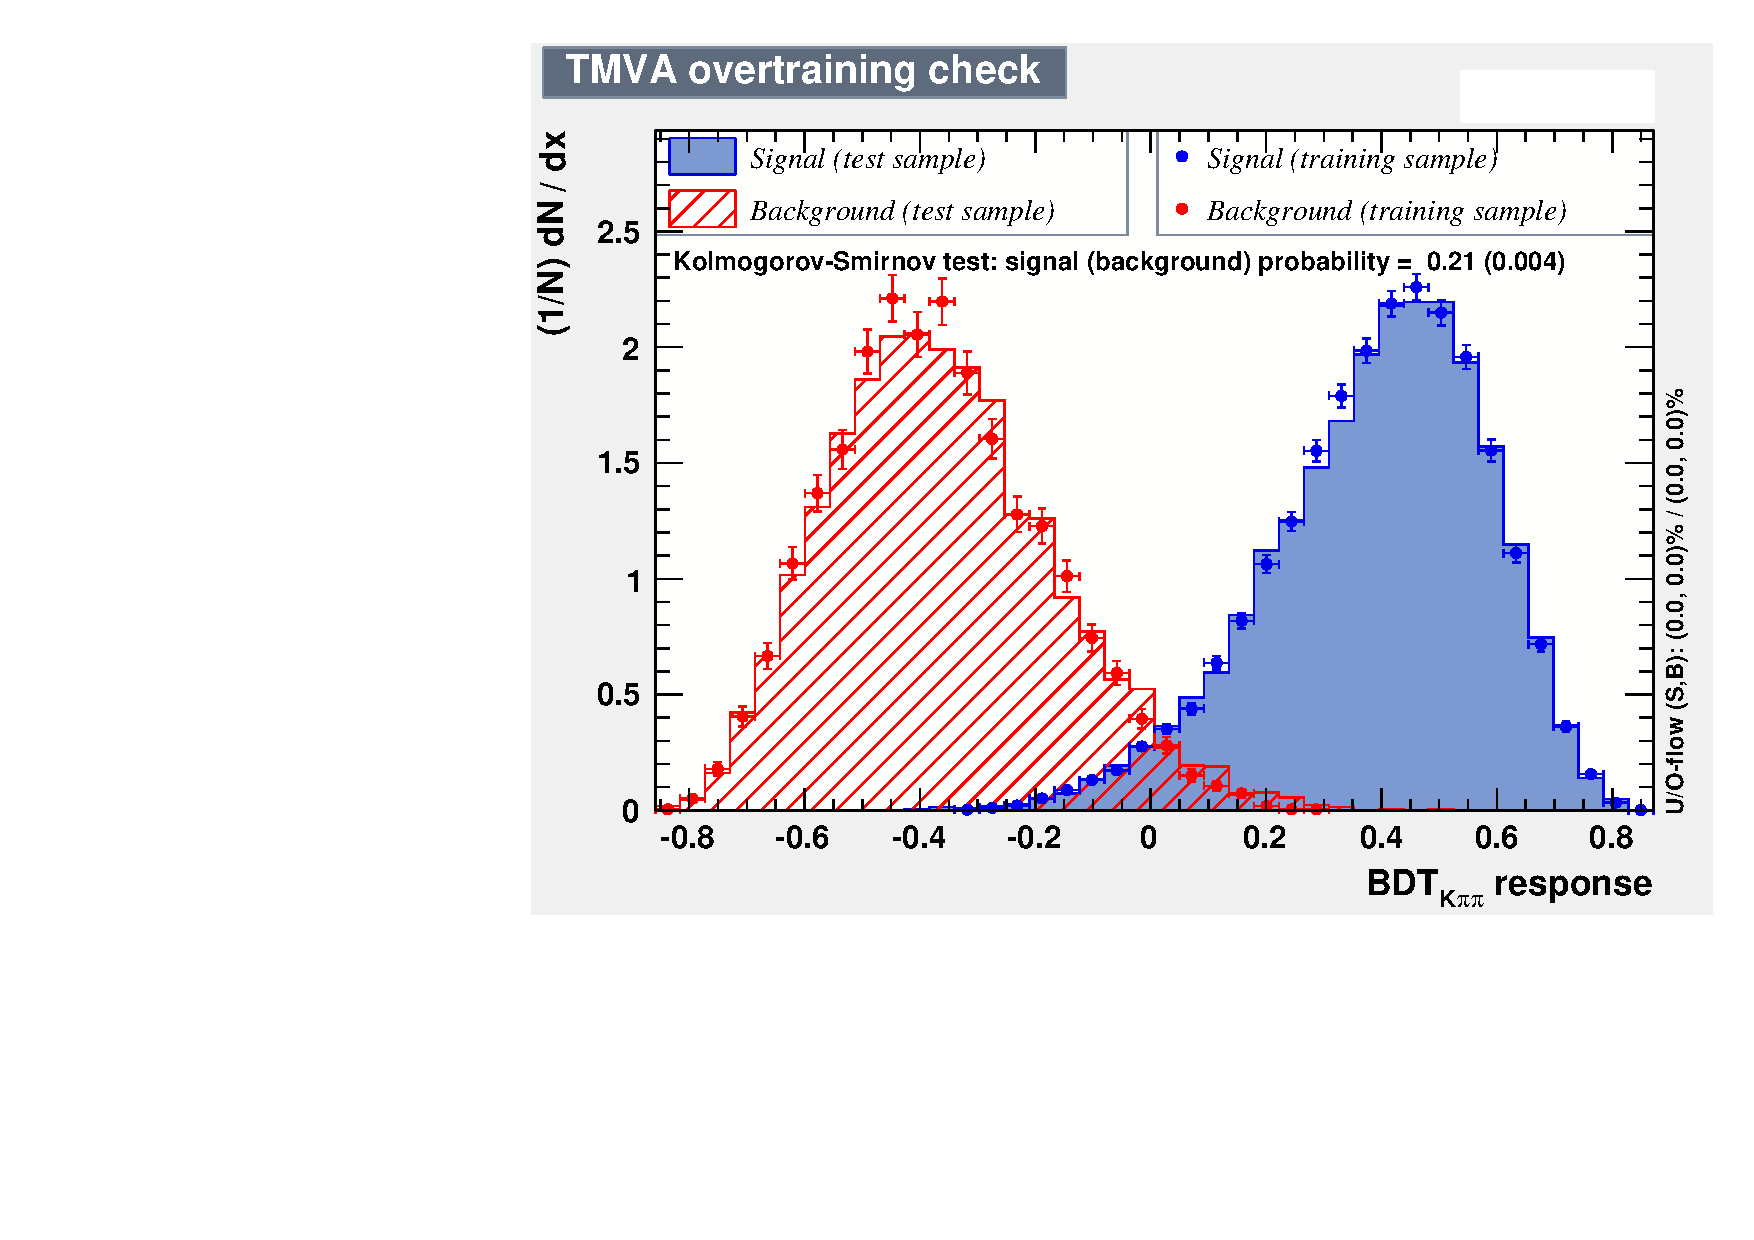
\includegraphics[width=0.48\textwidth]{07-B02DD/figs/Overtraining_Check_Kpipi.pdf}
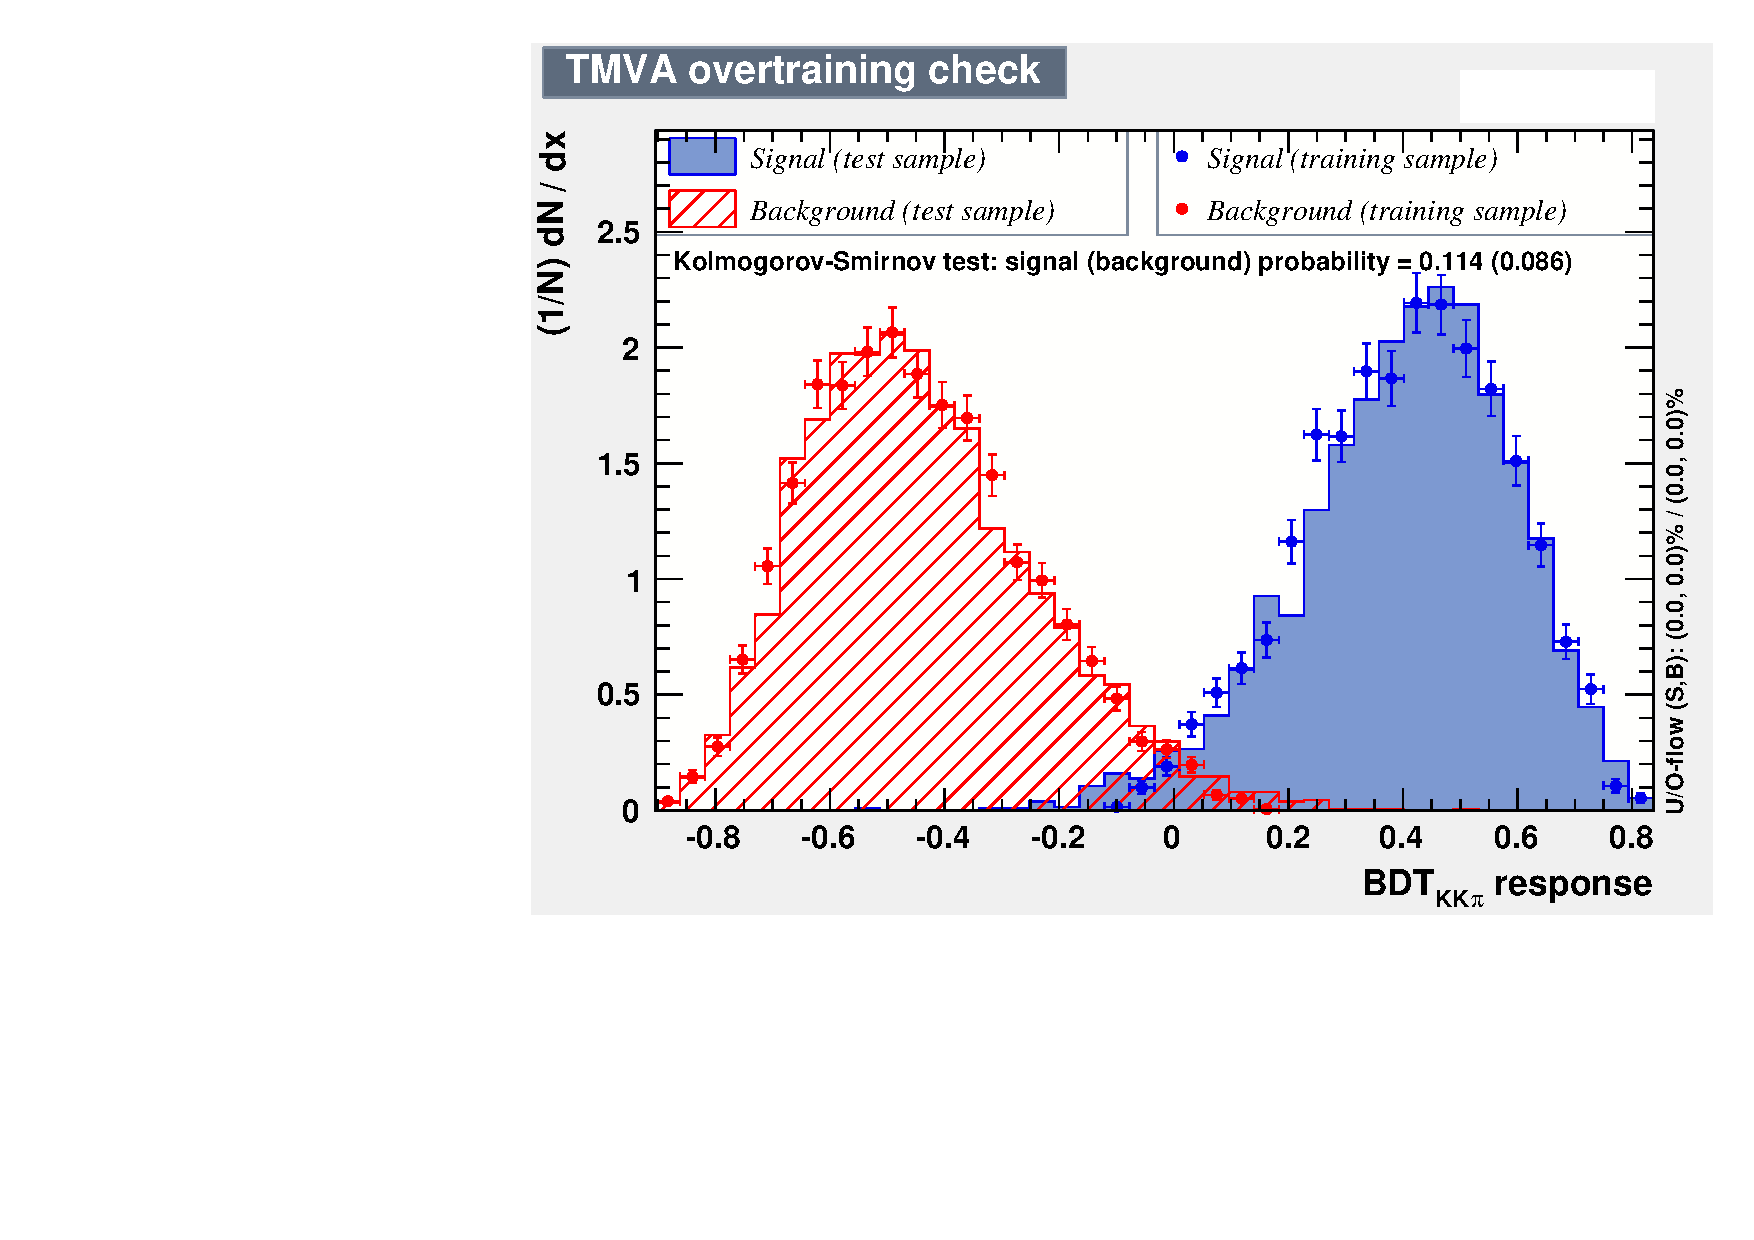
\includegraphics[width=0.48\textwidth]{07-B02DD/figs/Overtraining_Check_KKpi.pdf}
\caption{Comparison of the BDT response on training and test sample for the
\KpipiKpipi final state (left) and the \KKpiKpipi final state (right).}
\label{fig:b02dd:selection:mva:overtraining}
\end{figure}
%
Using simulations in the selection contains the possibility that certain
distributions are not modelled properly and differences between the simulation
and real data are exploited instead of differences between signal and
background. Indeed, the classifier output distributions of the signal MC and
background-subtracted data show a quite large disagreement for both final
states as can be seen in \cref{fig:b02dd:selection:mva:bdtcomparison}. The
performance is clearly overestimated in the training.
%
\begin{figure}[htbp]
    \centering
    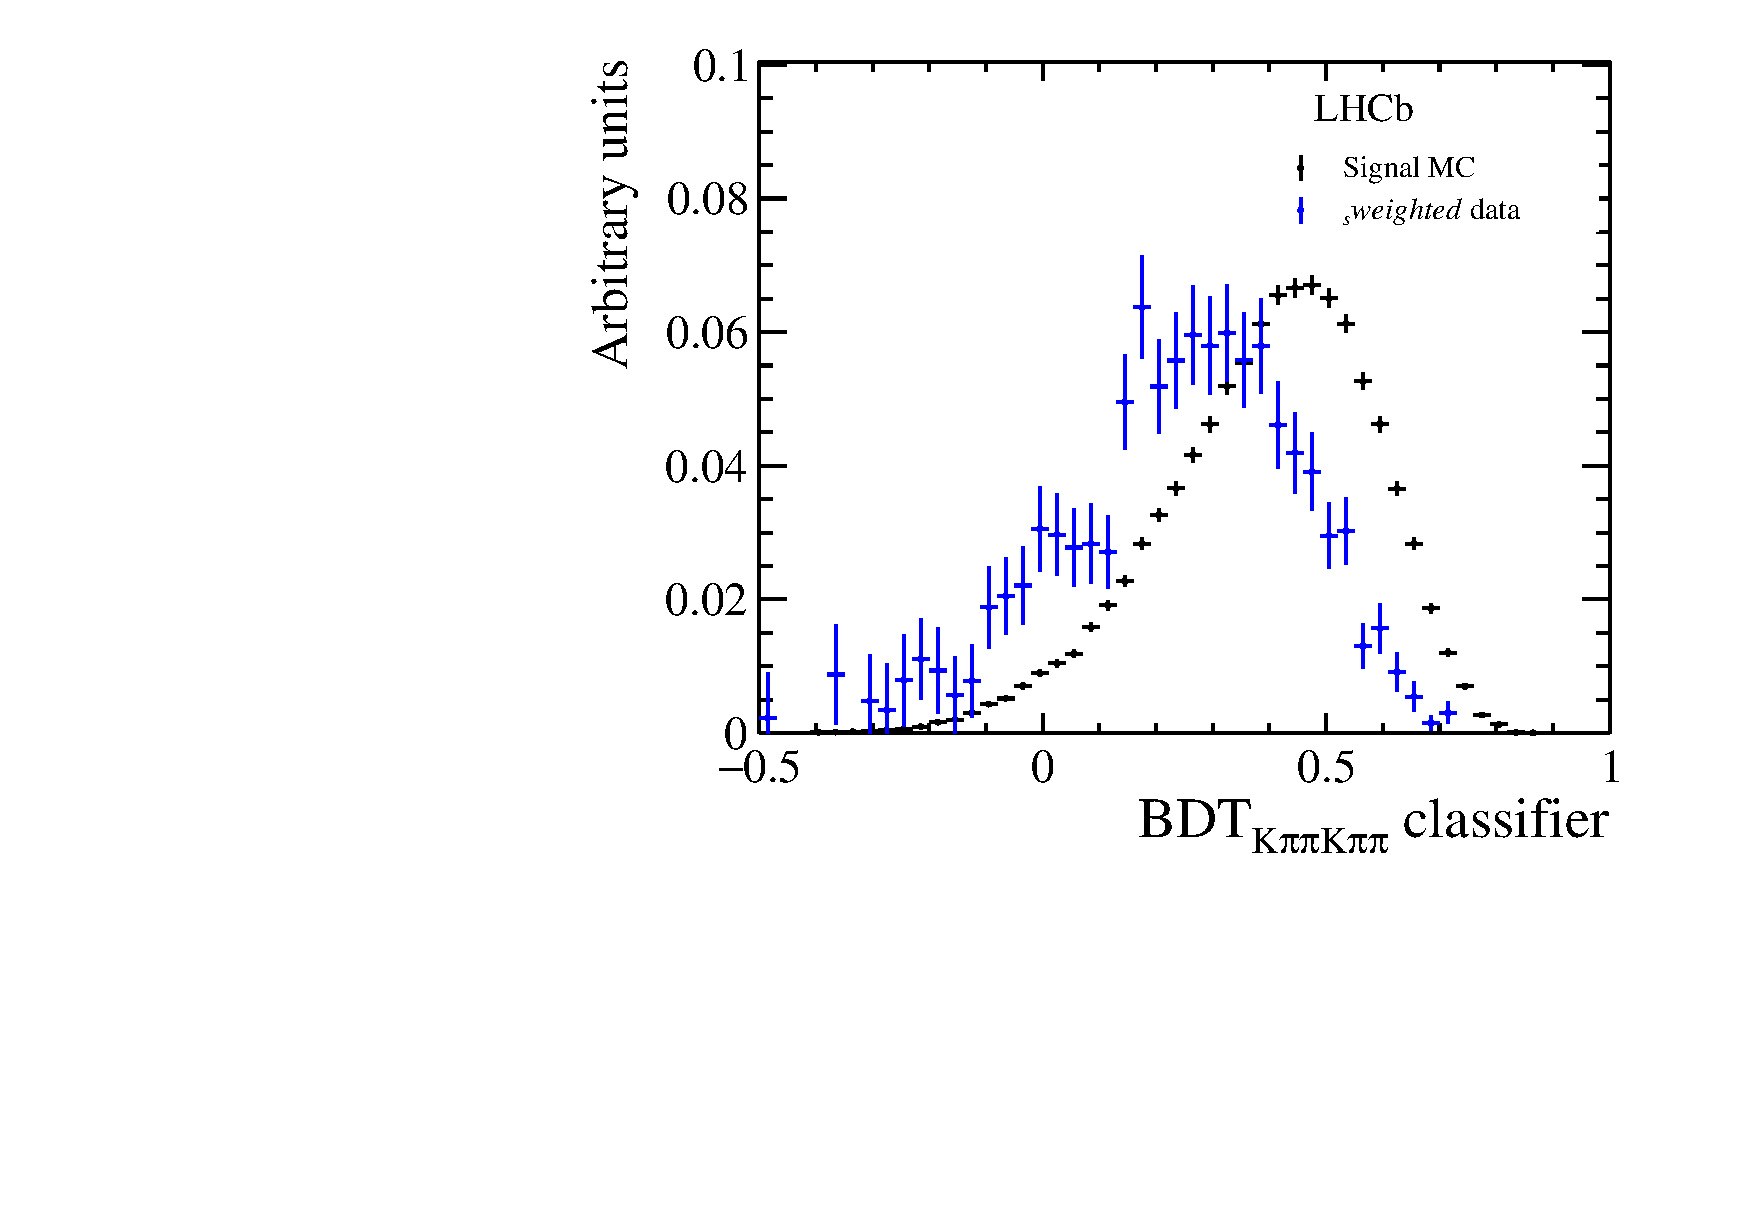
\includegraphics[width=0.49\textwidth]{07-B02DD/figs/BDTComparison_Kpipi.pdf}
    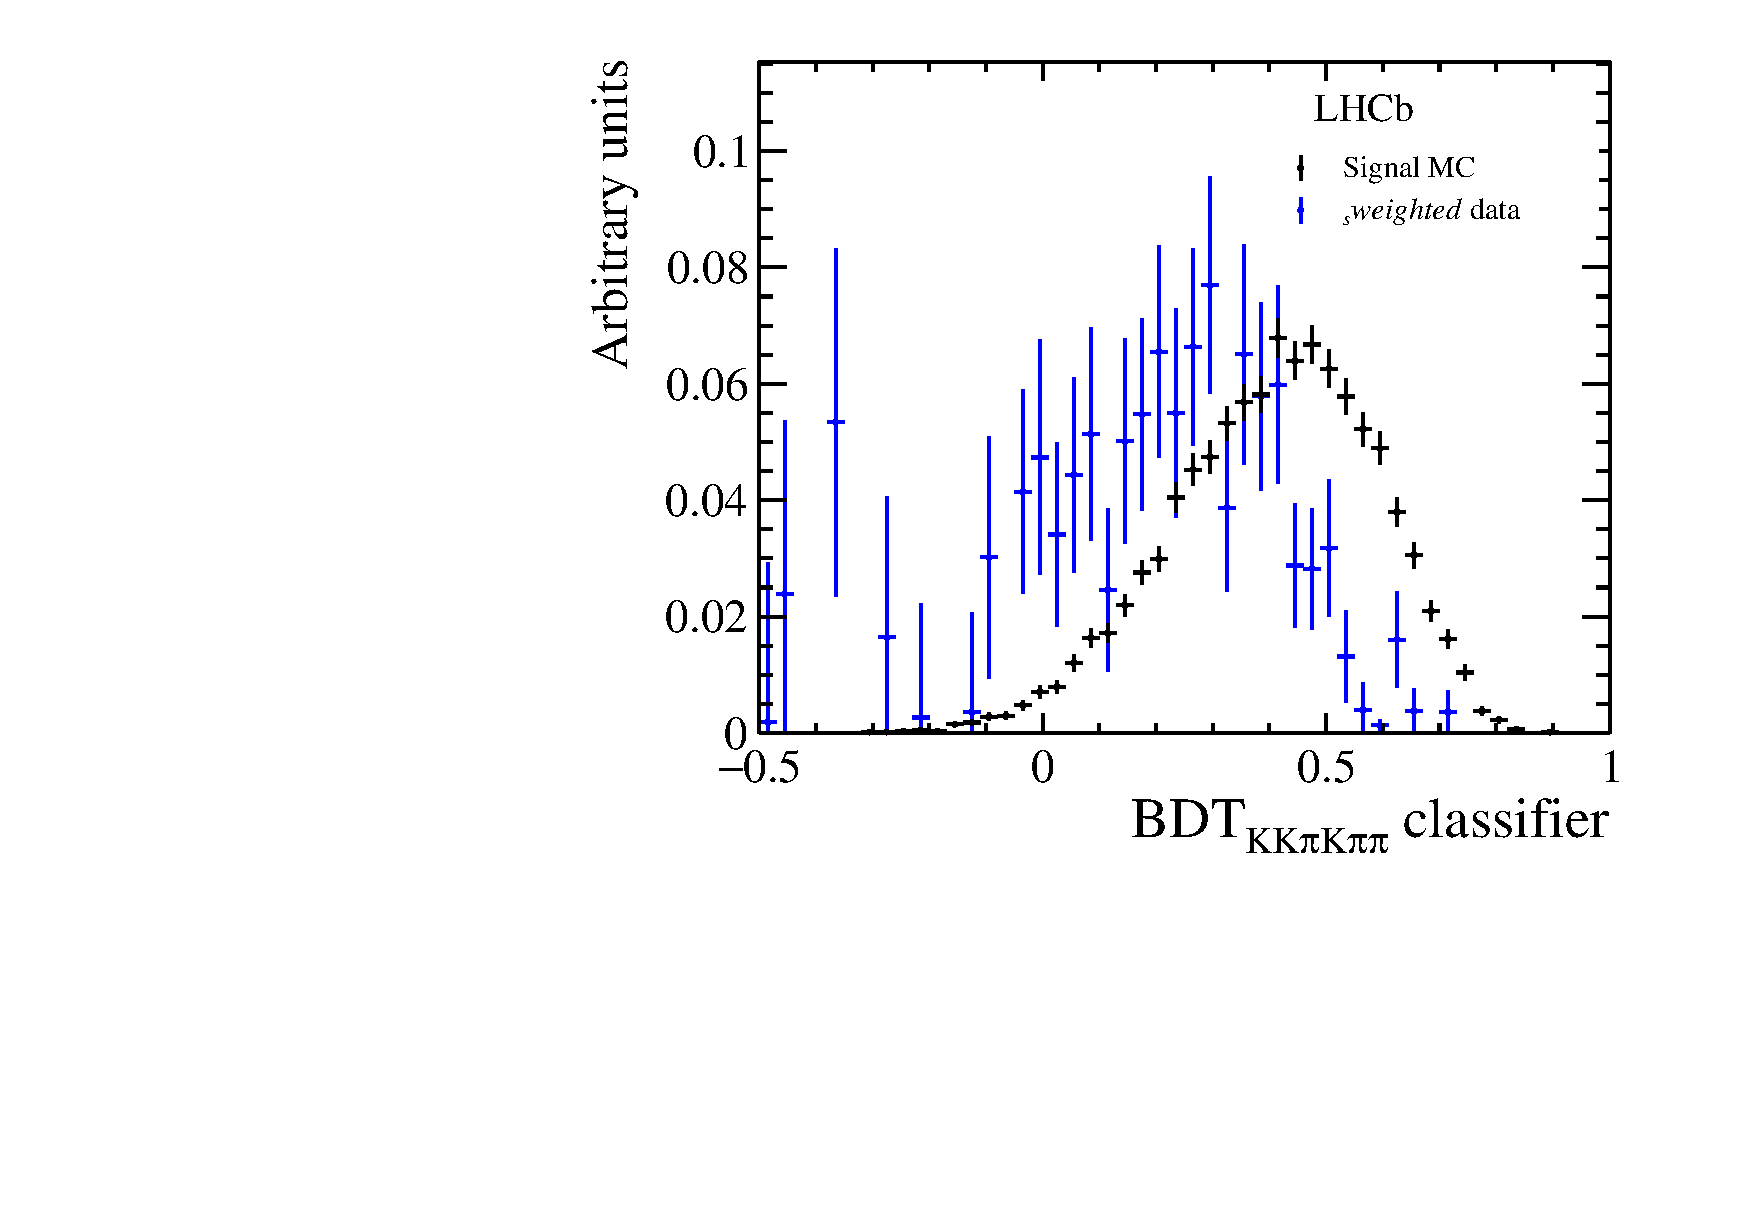
\includegraphics[width=0.49\textwidth]{07-B02DD/figs/BDTComparison_KKpi.pdf}
    \caption{Distribution of the BDT output for background-subtracted data (blue) and
    signal MC (black) for the \KpipiKpipi final state (left) and the
    \KKpiKpipi final state (right).}
    \label{fig:b02dd:selection:mva:bdtcomparison}
\end{figure}
%
This would be a problem if the selection efficiencies had to be calculated
using the MC sample. But for a measurement of \CP violation it is mainly
important that the amount of background can somehow be reduced while most of
the signal is kept. This can be achieved with the current setting.

% ==============================================================================
\subsubsection*{BDT cut optimisation}
\label{sec:b02dd:selection:mva:optimisation}

As explained in \cref{sec:dataanalysis:selection:fom} the best figure of merit
for a measurement of \CP violation is the sensitivity on the \CP observables
themselves. So the requirement on the BDT classifier output is scanned
performing a fit to the invariant $\Dp\Dm$ mass spectrum followed by a decay
time fit of the background-subtracted sample for each scan point. Initially,
only the subsample with two kaons in the \Bd final state is analysed. In
\cref{fig:b02dd:selection:mva:sensitivities} the statistical
uncertainties of \SDD and \CDD are plotted as a function of the requirement on
the BDT classifier output.
%
\begin{figure}[!htb]
\centering
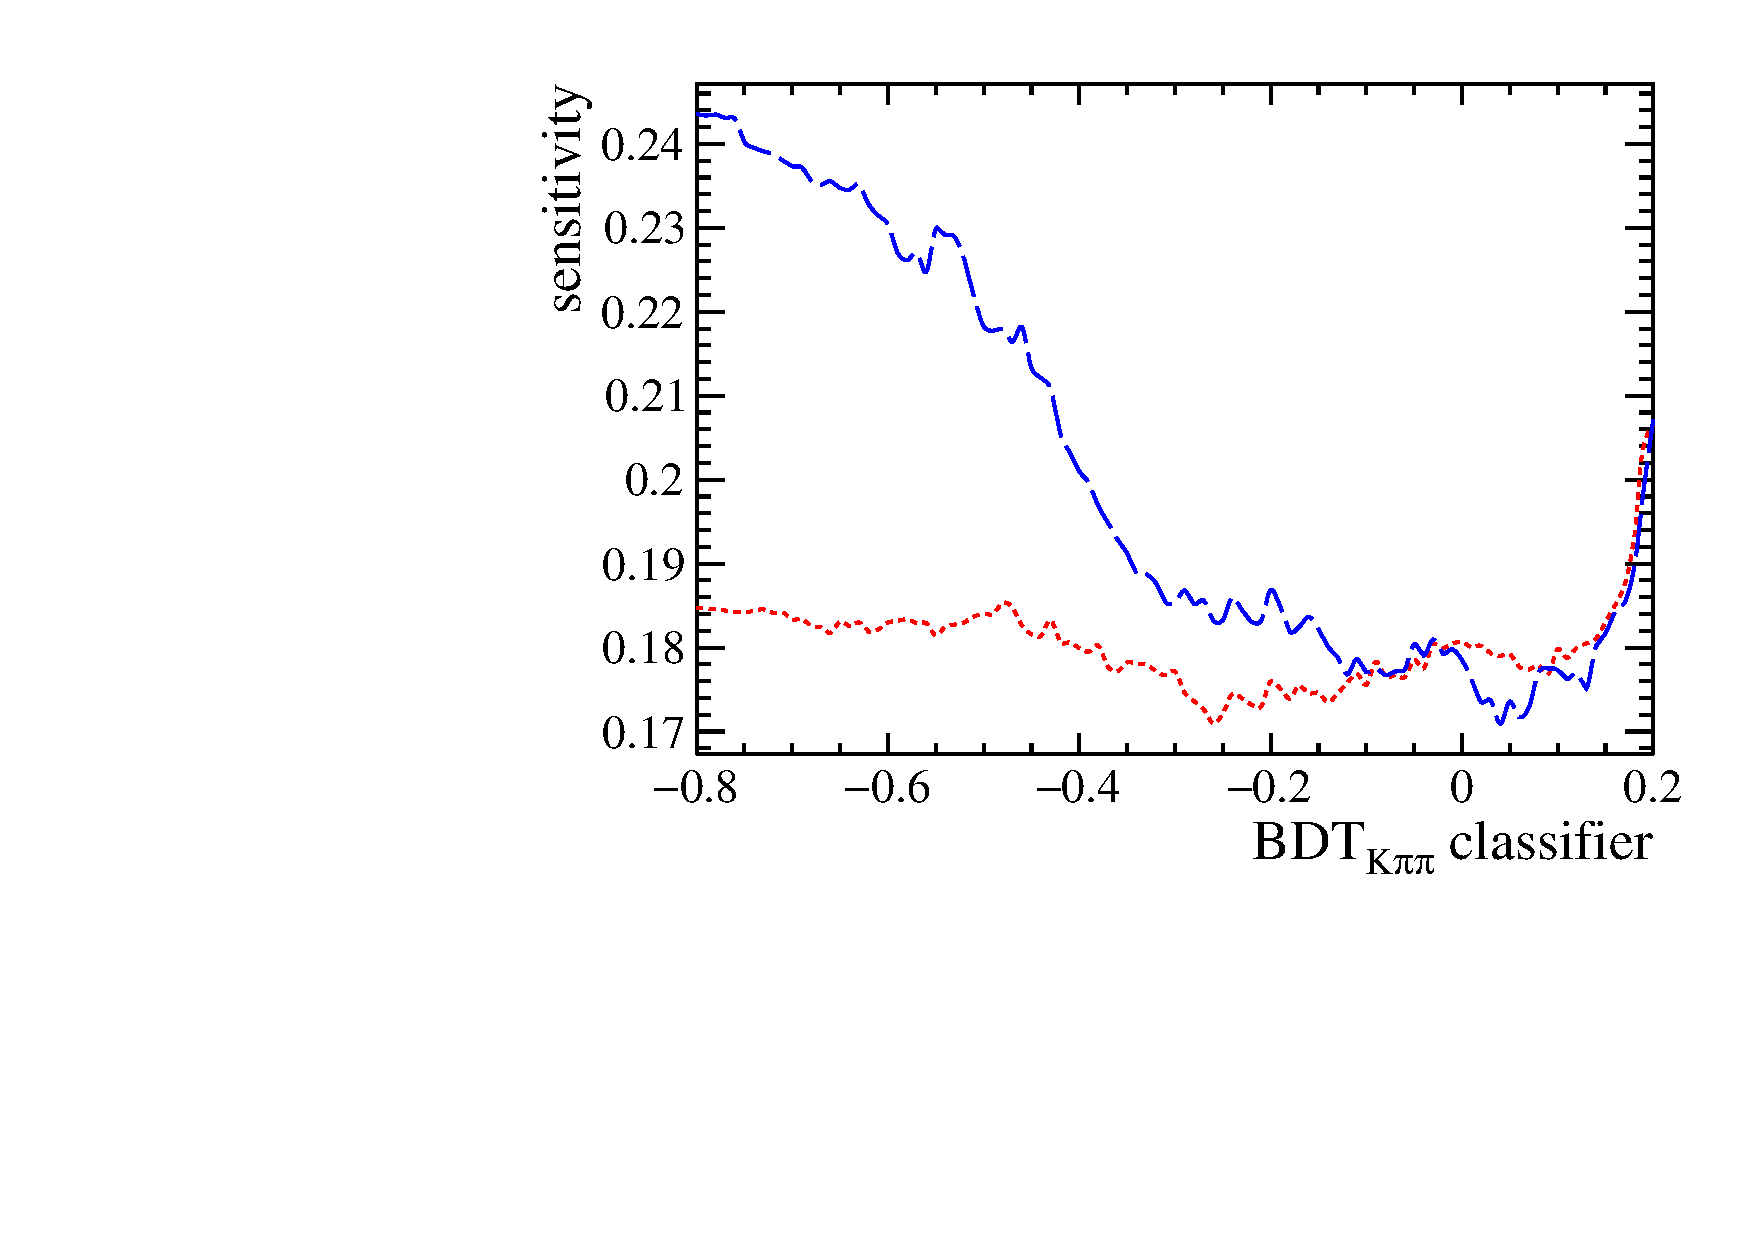
\includegraphics[width=0.48\textwidth]{07-B02DD/figs/Sensitivities_Kpipi.pdf}
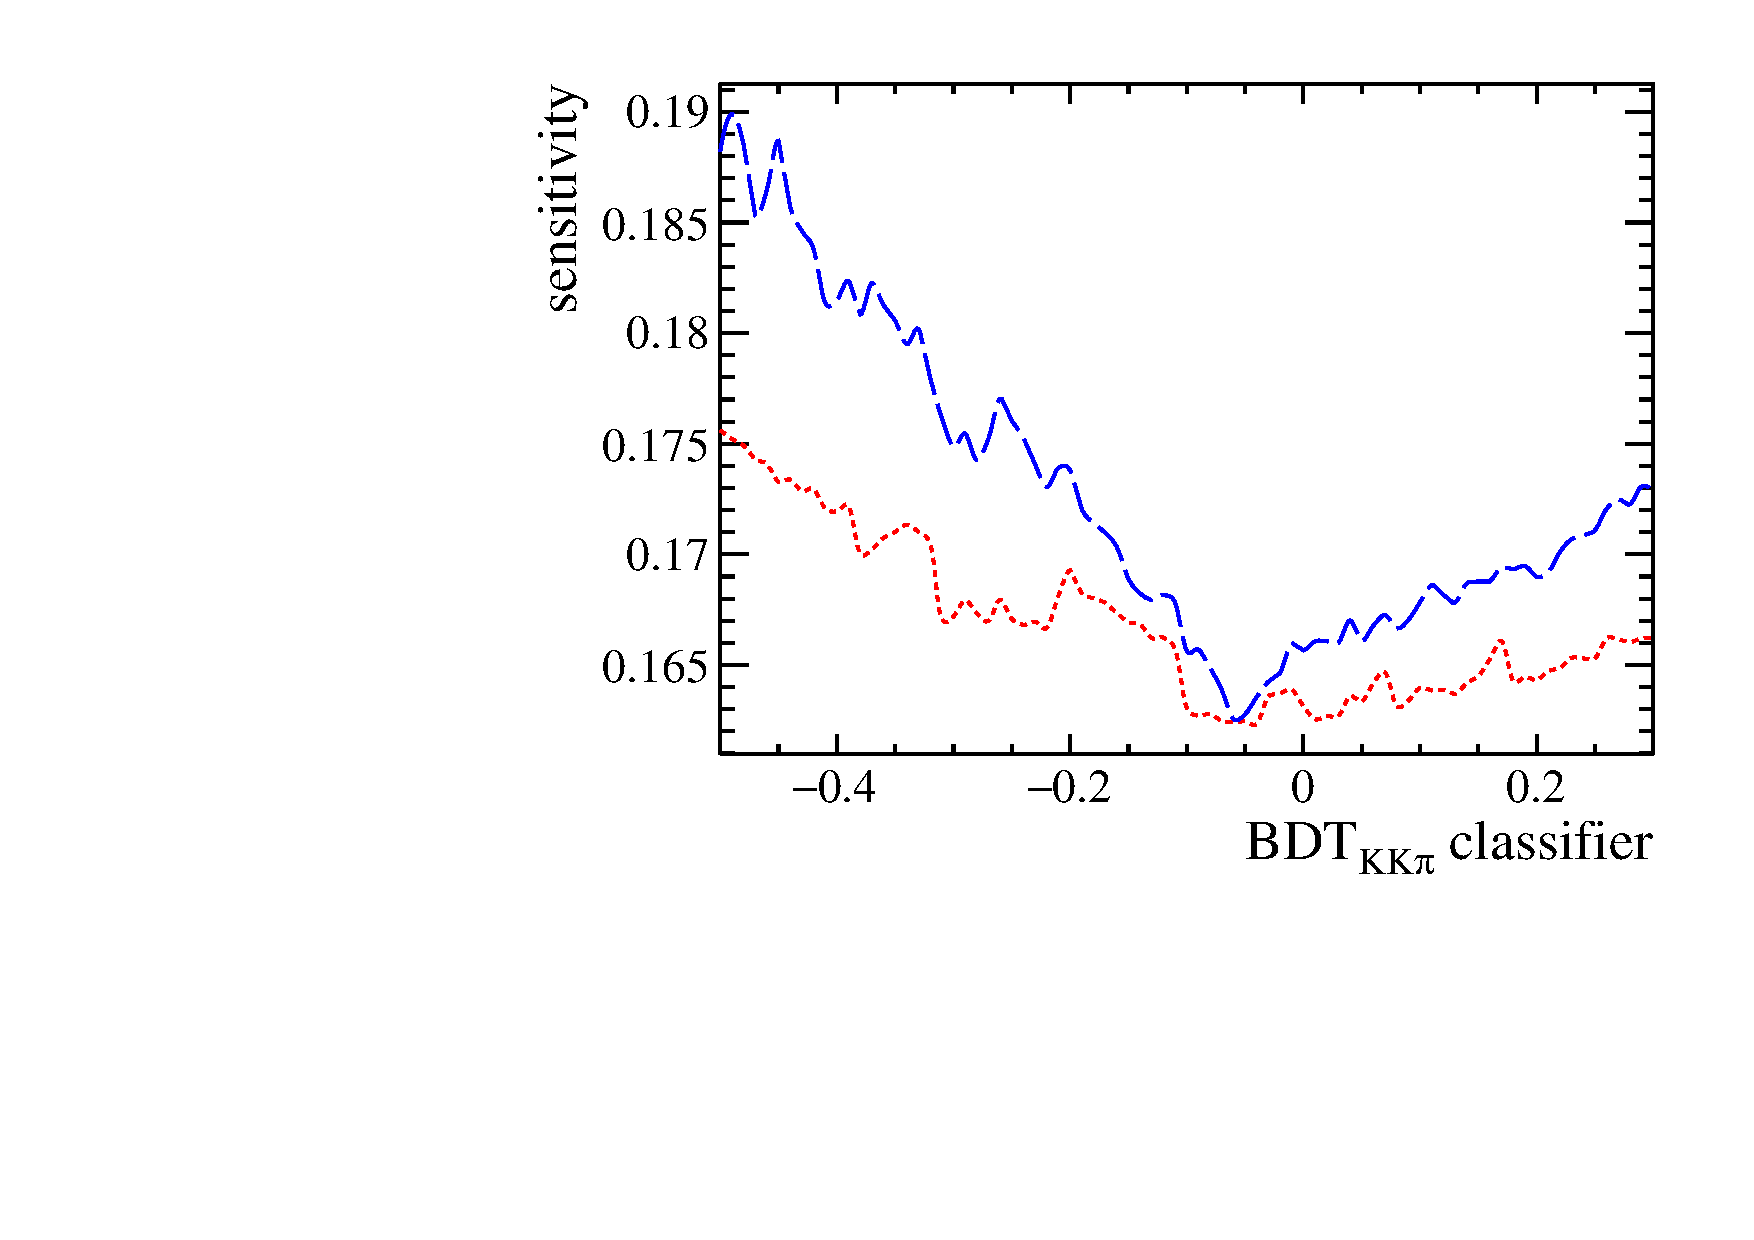
\includegraphics[width=0.48\textwidth]{07-B02DD/figs/Sensitivities_KKpi.pdf}
\caption{Sensitivity of \SDD (red short-dashed) and \CDD (blue long-dashed) as
a function of the BDT classifier output for the \KpipiKpipi final state (left)
and the \KKpiKpipi final state (right).}
\label{fig:b02dd:selection:mva:sensitivities}
\end{figure}
%
The uncertainty on \CDD improves with tighter requirements on the BDT
classifier until it reaches an optimum shortly after zero. This can be
explained with the fact that the sensitivity on \CDD mainly comes from
candidates at low decay times because the cosine function is maximal there.
The suppression of the rather short-lived combinatorial background compensates
the loss in signal efficiency for a quite long range. In contrast, the
uncertainty on \SDD is mainly driven by the amount of signal candidates. So it
is more or less flat for loose requirements on the BDT classifier where only
few signal candidates are lost and this is compensated by the higher purity
and reaches its optimum around \num{-0.25} before it starts to get worse. Now
that both observables are of interest and the optima are not at the same cut
value it is decided to require the BDT classifier to be greater than
\num{-0.10}. This is a good compromise between both observables as the
uncertainties of \SDD and \CDD are almost the same and close to their optima.
The requirement has a signal efficiency of \SI{96.5\pm0.5}{\percent} and
rejects \SI{84.18\pm0.34}{\percent} of the combinatorial background.

In a second step the requirement on the BDT classifier for the \KKpiKpipi
final state is optimised. The \KKpiKpipi subsample is quite small, which makes
individual fits on this subsample rather unstable. This can be solved by
performing a simultaneous fit to the whole dataset with the previously
determined BDT cut applied to the \KpipiKpipi subsample. Scanning the BDT
classifier output for the \KKpiKpipi final state results in the sensitivities
on \SDD and \CDD plotted in \cref{fig:b02dd:selection:mva:sensitivities}. Both
uncertainties show a minimum at around \num{-0.05}, which is chosen as cut
value. This cut removes \SI{90.75\pm0.33}{\percent} of the combinatorial
background at a signal efficiency of \SI{87.2\pm1.9}{\percent}.

\subsection{Final selection}
\label{sec:b02dd:selection:final_selection}

Finally, the fit range of the invariant $m_{\Dp\Dm}$ mass is reduced to
\SIrange{5150}{5500}{\MeVcc}, which eliminates some backgrounds, like
misreconstructed \mbox{\BdToDstD}, at low masses, prevents overtraining
effects on the high-mass sideband used in the training of the BDT, and leaves
enough candidates in the upper mass sideband to determine the shape of the
combinatorial background. Additionally, the decay time is restricted to be in
the range \SIrange{0.25}{10.25}{\ps} to avoid edge effects. In
\SI{0.8}{\percent} of the selected events more than one candidate remains,
which is very unlikely given the low branching branching fraction. So choosing
randomly only one of the multiple candidates is kept.


%!TEX root = ../main.tex

\section{Mass fit (5 pages)}
\label{sec:b02dd:massfit}

%!TEX root = ../main.tex

\section{Decay time fit}
\label{sec:b02dd:decaytimefit}

The conditional PDF describing the reconstructed decay time $t'$ and tag
decisions $\vect{d'} = (\dos, \dss)$, given a per-event decay time resolution
$\sigma_{t'}$ and per-event mistag probability estimates $\vect{\eta} = (\etaos,
\etass)$, is
%
\begin{equation}\label{eq:fullpdf}
  P\left(t',\vect{d'}\given \sigma_{t'},\vect{\eta}\right)
  \propto \epsilon(t') \left(\mathcal{P}(t,\vect{d'}\given \vect{\eta})
    \otimes \mathcal{R}(t'-t\given \sigma_{t'})\right)\,,
\end{equation}
%
where
\begin{equation}
  \mathcal{P}(t,\vect{d'}\given \vect{\eta}) \\
  \propto \sum_{d} \mathcal{P}(\vect{d'} \given d,\vect{\eta})
      [1 - d\, A_\text{P}] \,
      e^{-t/\tau}\left\{1 - d\, S \sin(\dm t) + d\, C \cos(\dm t)\right\}\,,
\end{equation}
and where $t$ is the true decay time, $d$ is the true production flavour,
$A_\text{P}$ is the production asymmetry, and $\mathcal{P}(\vect{d'} \given
d,\vect{\eta})$ is a two-dimensional binomial PDF describing the distribution
of tagging decisions given $\vect{\eta}$ and $d$. Normalisation factors are omitted for brevity.

%============================================================================%
%!TEX root = ../main.tex
\section{Decay time resolution}
\label{sec:dataanalysis::resolution}

Uncertainties in the determination of the position of vertices and in the
measurement of momenta (although thanks to the VELO (see
\cref{sec:detector:lhcb}) pretty accurate  at $\lhcb$) lead to a finite decay
time resolution $\sigma$, which dilutes the observed $\CP$ asymmetry by a
factor
\begin{align}
  \mathcal{D} = e^{\frac{-\dmd^2\,\sigma^2}{2}} \, .
\end{align}
This formula is the special case for a Gaussian resolution model with width
$\sigma$. The general formula is derived in
Ref.~\cite{ResolutionDilutionFactor}. For $\Bd$ mesons the dilution induced by
the decay time resolution has only minor influence on the measurement of $\CP$
observables because the oscillation frequency of $\Bd$ mesons $\dmd =
\SI{0.5064\pm0.0019}{\hbar\invps}$~\cite{HFAG} is quite low. Even for a decay time
resolution of \SI{100}{\fs}, which would be almost two times larger than what
is usually found in analyses performed by \lhcb, the dilution factor is
greater than \SI{99}{\percent}.

\FloatBarrier
%============================================================================%
%!TEX root = ../main.tex
\subsection{Decay time acceptance}
\label{sec:b02dd:decaytimefit:acceptance}

The trigger requirements as well as some input variables to the BDT result in
a decay-time-dependent efficiency. Additionally, the \velo reconstruction
(\ie the FastVelo algorithm~\cite{Callot:2011bza}) causes a drop in decay time
acceptance for events with large decay times. In order to correctly describe
these effects the $\Bd$ lifetime is constrained to its PDG value of $\tau =
\SI{1.519\pm0.005}{\ps}$~\cite{PDG2014} in the nominal fit and any deviation
of the decay time distribution (summed over the tags) from a pure exponential
shape is supposed to be described by cubic splines (see
\cref{sec:dataanalysis:splines}). Knots are positioned on the rising edge,
approximately at the turning point, and at the boundaries of the decay time
range, so at $\{\SIlist[list-final-separator={,
}]{0.25;0.8;2.0;10.25}{\ps}\}$. The normalisation of the splines is arbitrary
and it has been decided to fix the second to last spline coefficient to
$\num{1.0}$.

On signal MC the truth information is available so the shape of the decay time
acceptance can be separated from the exponential decay. This shape is compared
with the spline method described above. As the BDTs are trained and applied
separately for the two final states and might have different effects on the
shape of the decay time acceptance these two categories are studied
individually.

\begin{figure}[htb]
\centering
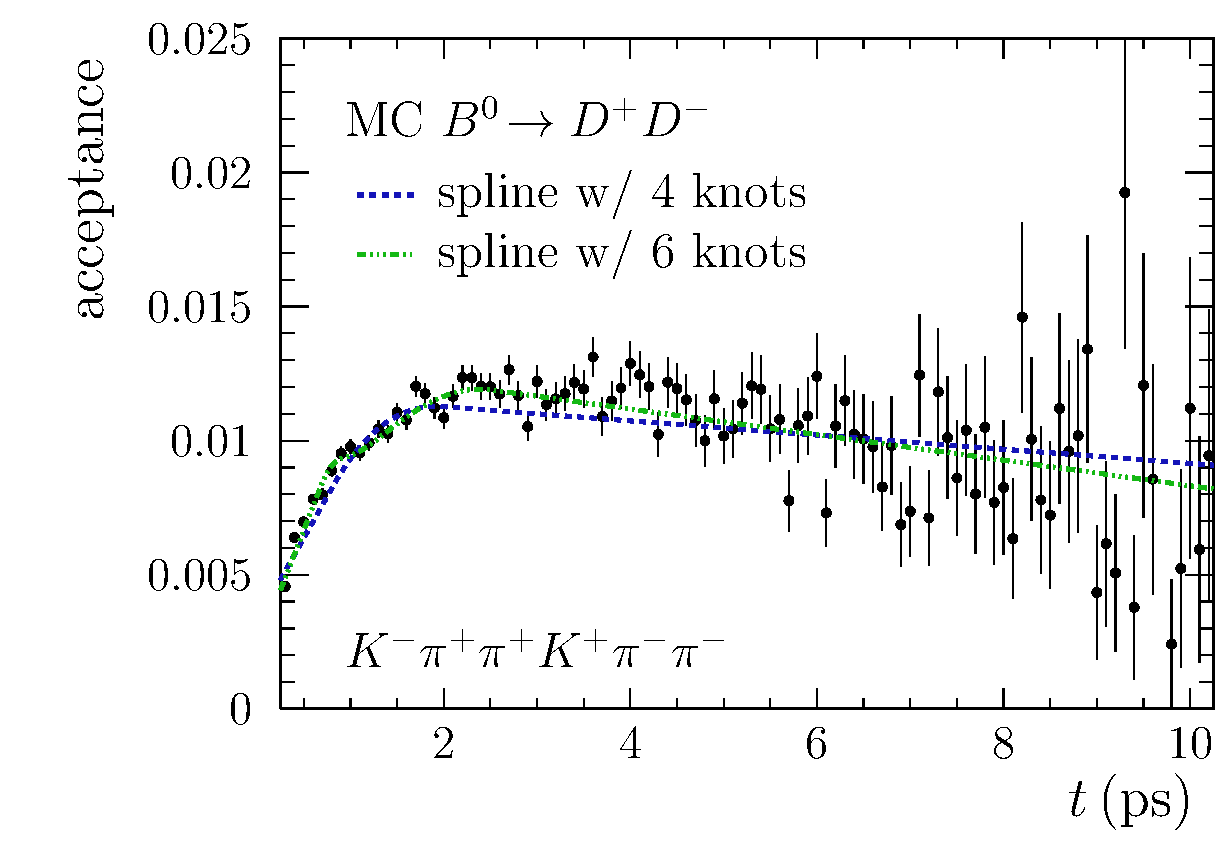
\includegraphics[width=0.48\textwidth]{07-B02DD/tikz/pdf/Acceptancespline_nolog_MC_Kpipi.pdf}
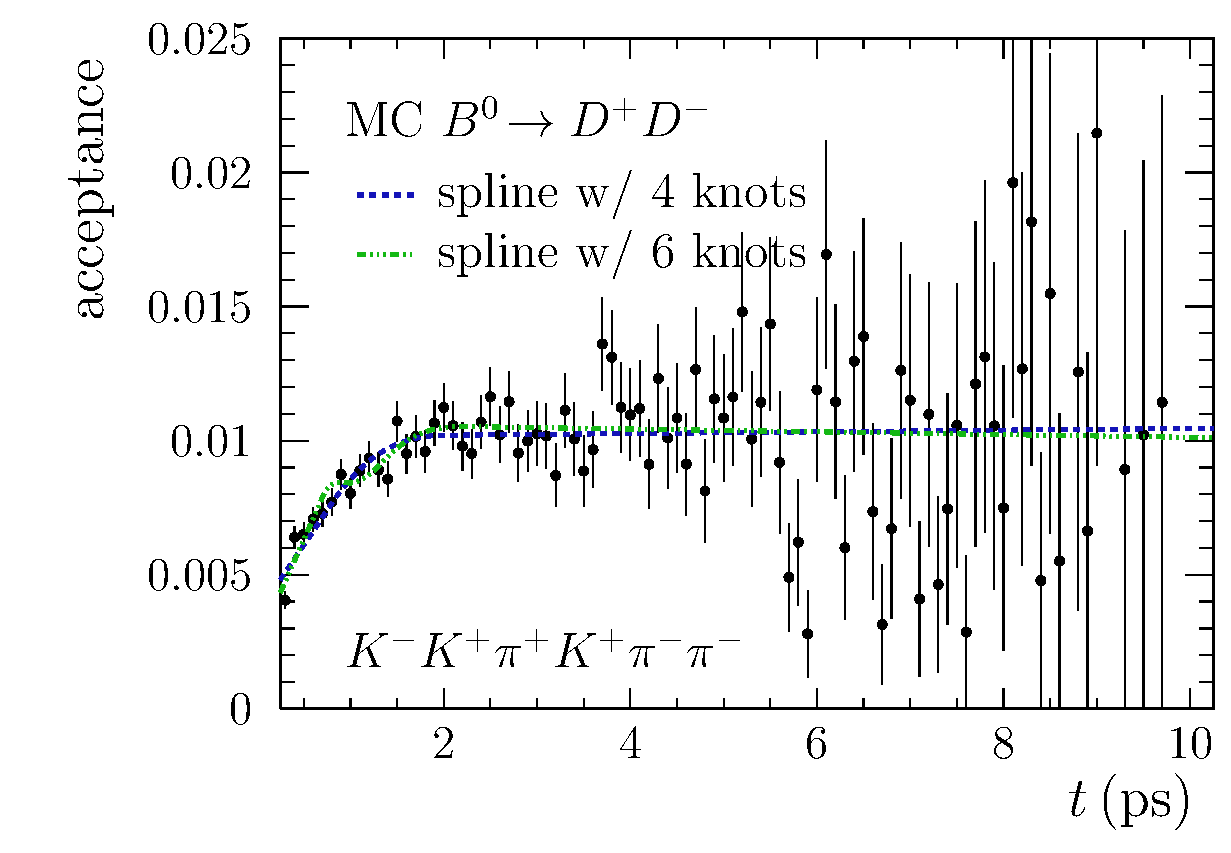
\includegraphics[width=0.48\textwidth]{07-B02DD/tikz/pdf/Acceptancespline_nolog_MC_KKpi.pdf}
\caption{Decay time acceptance of truth-matched signal MC for the $\KpipiKpipi$
final state (left) and the $\KKpiKpipi$ final state (right). The black data
points show the true decay time acceptance determined by dividing the
reconstructed by the true decay time distribution. The blue line is the spline
acceptance function and the red stripes indicate the $1\,\sigma$ error band
taking into account the statistical uncertainties.}
\label{fig:b02dd:decaytimefit:acceptance_MC}
\end{figure}

Looking at the plots in \cref{fig:b02dd:decaytimefit:acceptance_MC} it is
apparent that compared to $\BdToJPsiKS$ there is a quite large efficiency loss
at high decay times. This might be related to the fact that both $\Bd$
daughter particles ($\Dp$ and $\Dm$) are relatively long-lived. The true MC
decay time acceptance is overlaid with the shape of two spline functions.
Besides the spline function with the nominal number of four knots an
additional spline function with two more knots and slightly changed positions
$(\SIlist[list-final-separator={, }]{0.25;0.7;1.0;1.5;2.5;10.25}{\ps})$ is
plotted, which gives a better description. But it has to be considered that
the statistics of the MC sample is \num{25} times larger than the real data.
Therefore, the spline function with four knots is chosen, otherwise rather
statistical fluctuations than acceptance effects would be described. The low
statistics of the $\KKpiKpipi$ final state on real data does also not allow to
use separate spline coefficients for the two final states although with the
increased MC statistics some differences become visible.


\FloatBarrier
%============================================================================%
\subsection{External inputs}
\label{sec:b02dd:decaytimefit:constraints}

\lhcb has performed a measurement of the production asymmetry as a function
of transverse momentum and pseudorapidity using \SI{7}{\TeV}
data~\cite{LHCb-PAPER-2014-042}. Taking those distributions from \BdToDD
individual weighted averages for the 2011 and 2012 subsamples are calculated
yielding
%
\begin{equation}
  \begin{split}
    \prodasym{11} &= -0.0047 \pm 0.0106 \,\text{(stat)} \pm 0.0014 \, \text{(syst)} \,, \\
    \prodasym{12} &= -0.0071 \pm 0.0107 \,\text{(stat)} \pm 0.0014 \, \text{(syst)} \,.
  \end{split}
\end{equation}
%
As the measurement of the production asymmetry has been performed on 2011 data
only, the numbers for $\prodasym{11}$ and $\prodasym{12}$ are highly
correlated. So, the latter is modelled as $\prodasym{12} = \prodasym{11} +
\Delta\prodasym{}$ with $\Delta\prodasym{} = -0.0024 \pm 0.0018
\,\text{(syst)}$. The systematic uncertainty accounts for the difference of
the production asymmetries observed for the two data-taking conditions in the
measurement of the semileptonic $\CP$ asymmetry~\cite{LHCb-PAPER-2014-053} and
is used as the width of a Gaussian constraint. The $\Bz$ oscillation frequency and
the $\Bz$ lifetime are constrained to $\dm =
\SI{0.510\pm0.003}{\planckbar\invps}$~\cite{PDG2014} and $\tau =
\SI{1.519\pm0.005}{\ps}$~\cite{PDG2014}, respectively. The
flavour-tagging calibration parameters
(\cref{tab:dataanalysis:taggingcalibration:dsdcalibration}) are constrained
within their combined statistical and systematic uncertainties, determined in
the calibration using \BdToDsD decays. The decay time resolution parameters
(\cref{tab:b02dd:decaytimefit:resolution}) and the $\Bz$ lifetime difference
$\DG = \SI{0}{\invps}$ are fixed in the likelihood fit.

%============================================================================%
\subsection{Results}

The fit results of the $\CP$ observables from the decay time fit are
\begin{align}
\begin{split}
  \SDD                &= -0.54\,\pm\,^{0.17}_{0.16} \, , \\
  \CDD                &= \phantom{-}0.26\,\pm\,0.17 \, , \\
  \rho(\SDD,\CDD)     &= \phantom{-}0.48 \, . \\
\end{split}
\label{eq:b02dd:decaytimefit:cpresults}
\end{align}

Only after rescaling the sWeights via
\begin{align}
  w_i = w_i \frac{\sum w_i}{\sum w_i^2}\,,
\end{align}
correct asymmetric uncertainty estimates are delivered by \minos, which is
\root's standard method to analyse the likelihood shape. To check if the
coverage is guaranteed the bootstrapping method is applied. The nominal fit
procedure, \ie performing the mass fit, calculating the sWeights and fitting
the weighted tagged decay time distribution, is executed and the fit results
are stored. The drawing and fitting is done \num{10000} times. It turns out
that half of the fits fail if the flavour-tagging calibration parameters are
constrained within their statistical uncertainties. When fixing them to their
central values the fit failure rate drops to a per-mille effect. From the
distribution of fit results the two-side \SI{68}{\percent} confidence
intervals are extracted. To account for the uncertainties on the
flavour-tagging calibration parameters \num{10000} pseudoexperiments are
performed, in which the nominal model is used to generate the signal decay
time distribution and the fit results of the nominal fit are chosen for the
\CP observables \SDD and \CDD. Before generating the flavour-tagging
calibration parameters are drawn from Gaussian distributions around their
central values using the combined statistical + systematic uncertainties. In
the subsequent fit the flavour-tagging calibration parameters are fixed to
their central values, like in the fits to the bootstrapped samples. The
resulting pull distributions are broader than standard normal distributions.
The deviation of the width from unity shows how much the statistical
uncertainties are underestimated in the likelihood fit due to not accounting
for the variation of the flavour-tagging calibration parameters. So, the
statistical uncertainties for \SDD and \CDD from the bootstrapping including
the impact of the uncertainty of the flavour-tagging calibration parameters
are given by scaling the bootstrapping uncertainties by the width of the pull
distributions:
\begin{align}
    \sigma_{\SDD}(\text{bootstrapping}) &= \,^{+0.17}_{-0.16} \,, \\
    \sigma_{\CDD}(\text{bootstrapping}) &= \,^{+0.18}_{-0.17} \,.
\end{align}
These uncertainties match the nominal ones from \minos quite well. A plot of
the decay time distribution and the projection of the acceptance model are
shown in \cref{fig:b02dd:decaytimefit}. Good agreement between the latter and
the shape on signal MC (cf. \cref{fig:b02dd:decaytimefit:acceptance_MC}) can
be observed but the low statistics leading to rather large uncertainties
indicated by the error band diminishes the significance of the comparison.

\begin{figure}[htb]
\hspace*{\fill}
\begin{minipage}{0.4\textwidth}
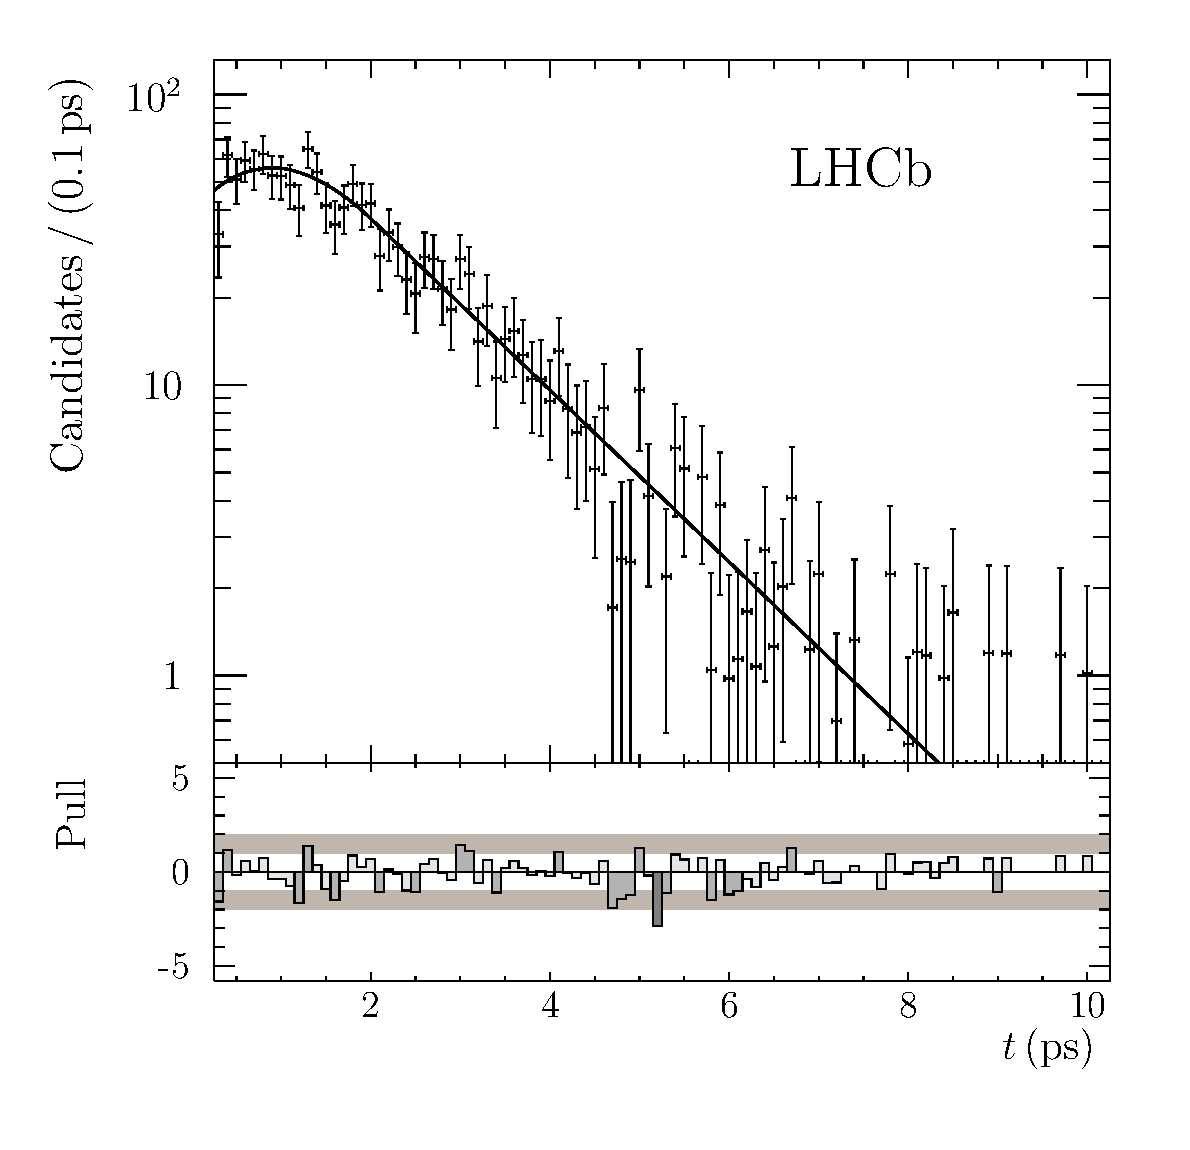
\includegraphics[width=\textwidth]{07-B02DD/tikz/pdf/obsTime_summed_pull_logy.pdf}
\end{minipage}
\hfill
\begin{minipage}{0.5\textwidth}
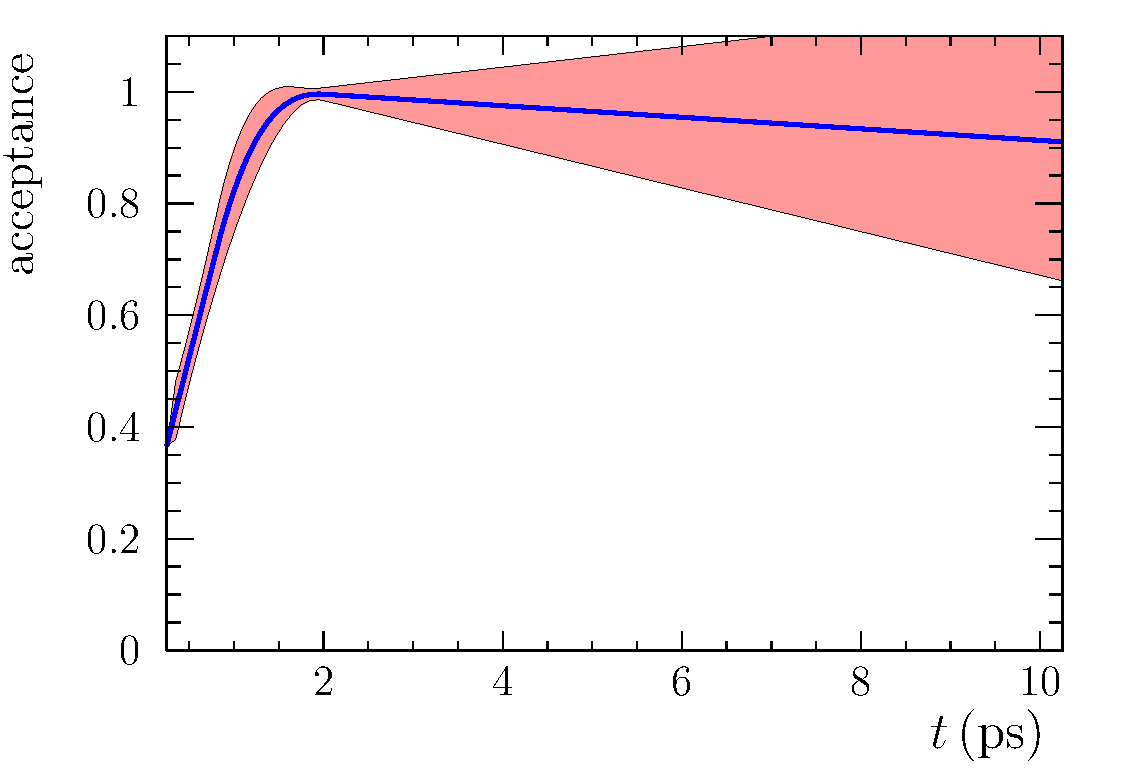
\includegraphics[width=\textwidth]{07-B02DD/tikz/pdf/Acceptancespline_nolog.pdf}
\end{minipage}
\hspace*{\fill}
\caption{Plot of the decay time distribution of the background-subtracted \BdToDD
data sample with the projection of the \PDF and the pull distribution on the
left. The y-axis is plotted in logarithmic scale. Plot of the nominal decay
time acceptance model on the right. The red area indicates the 1\,$\sigma$
error band taking into account the statistical uncertainties.}
\label{fig:b02dd:decaytimefit}
\end{figure}

Apart from a quite high positive correlation between the parameters of the
acceptance spline function and the already quoted correlation of about
\num{0.5} between $\SDD$ and $\CDD$, which is expected from first principles
(see Ref.~\cite{LHCb-ANA-2011-004}), no large correlation between fitted parameters
is present as can be seen from the correlation matrix visualised in
\cref{fig:b02dd:decaytimefit:FullFitCorrMatrixHotCold}. A possible correlation
between $\dm$ and $\CDD$ is significantly reduced by the constraint applied on $\dm$,
which is a lot tighter than the sensitivity accessible from the data sample.
When releasing this constraint the correlation coefficient becomes \num{-0.8}.
But the sensitivity on $\CDD$ would significantly decrease in this scenario, so
the constraint on $\dm$ is maintained in the nominal setup.

\begin{figure}[htb]
\centering
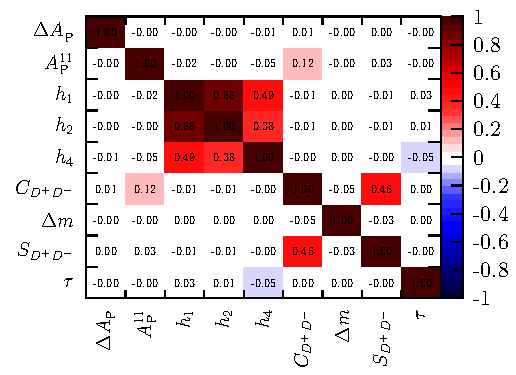
\includegraphics[width=0.5\textwidth]{07-B02DD/tikz/pdf/FitResultsCorrMatrix_RedBlueDiscrete_wText.pdf}
\caption{Visualised correlation matrix of the fit parameters in the decay time
fit to data. Positive correlations are represented by the red palette on the $z$ axis,
while negative correlations are represented by the blue palette of the $z$
axis.}
\label{fig:b02dd:decaytimefit:FullFitCorrMatrixHotCold}
\end{figure}

The 1D likelihood scans in \cref{fig:b02dd:decaytimefit:1DLLScan} show a nice
parabolic shape with a clear minimum.
\begin{figure}[htb]
\centering
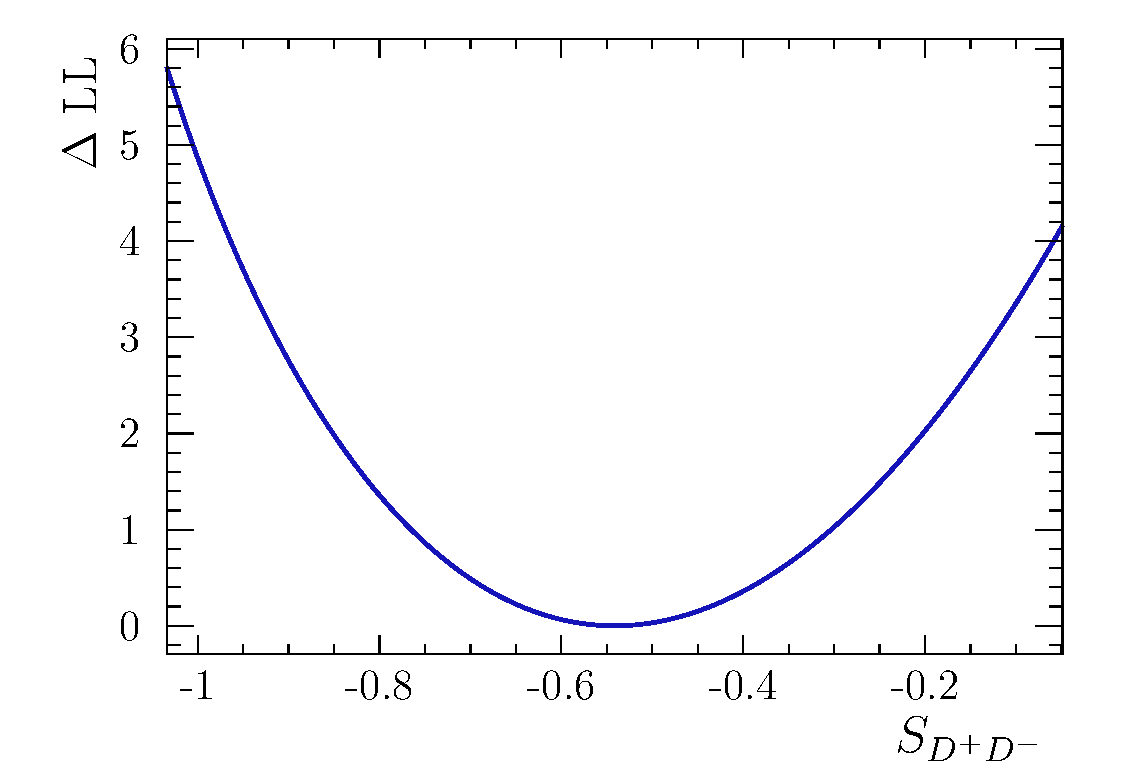
\includegraphics[width=0.48\textwidth]{07-B02DD/tikz/pdf/Likelihoodscan_sin2b.pdf}
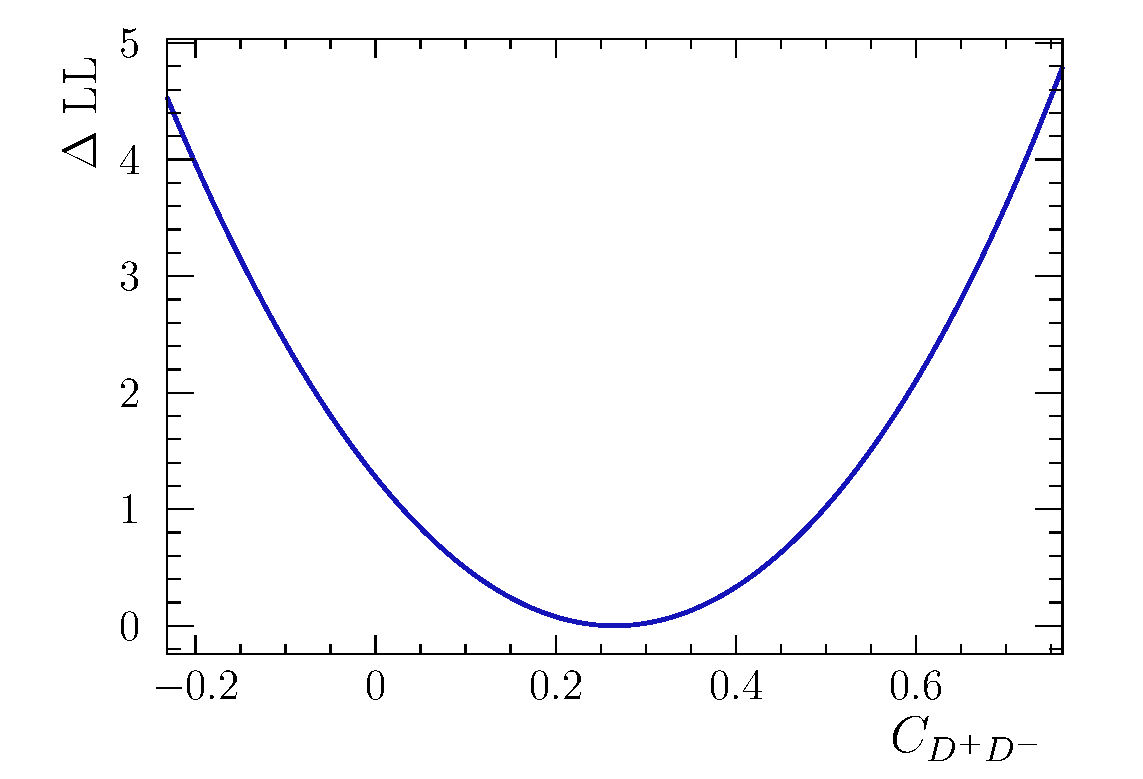
\includegraphics[width=0.48\textwidth]{07-B02DD/tikz/pdf/Likelihoodscan_C.pdf}
\caption{One-dimensional likelihood profile scans for $\SDD$ and $\CDD$.}
\label{fig:b02dd:decaytimefit:1DLLScan}
\end{figure}

In \cref{fig:b02dd:decaytimefit:asymmetry} the signal yield asymmetry is
plotted in eight bins of the decay time. A binned $\chisq$-fit to this signal
asymmetry is performed using
\begin{align}
{\mathcal A}^{\text{meas}}(t) = \frac{\Delta\omega + \prodasym{11}(1 - 2\omega) + (1 - 2\omega + \prodasym{11}\Delta\omega){\mathcal A}^{\text{theo}}(t)}{1 + \prodasym{11}(\SDD \sin(\dm\,t) - \CDD \cos(\dm\,t))}\,,
\label{eq:b02dd:decaytimefit:asymmetry_td}
\end{align}
which is a modified version of the theoretical signal asymmetry in
\cref{eq:cpviolation:simpleasymmetry} and accounts for the mistag probability
\mistag and the asymmetries induced by flavour tagging ($\Delta\omega$) and
production asymmetry ($\prodasym{11}$). The fit results
\begin{align*}
\begin{split}
  \SDD                &= -0.65\,\pm\,0.25 \,, \\
  \CDD                &= \phantom{-}0.24\,\pm\,0.26 \,,
\end{split}
\end{align*}
are compatible with those from the unbinned fit presented in
\cref{eq:b02dd:decaytimefit:cpresults} but not as sensitive.
\begin{figure}[htb]
\centering
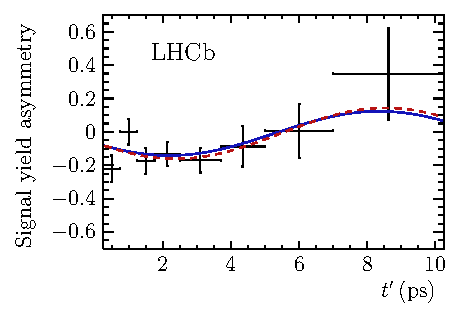
\includegraphics[width=0.48\textwidth]{07-B02DD/tikz/pdf/Asymmetry.pdf}
\caption{Decay-time-dependent signal yield asymmetry. The solid blue curve is the
projection of the signal PDF given in \cref{eq:fullpdf} and the dashed red curve is the
pure time-dependent fit function from
\cref{eq:b02dd:decaytimefit:asymmetry_td}}
\label{fig:b02dd:decaytimefit:asymmetry}
\end{figure}

\FloatBarrier


%!TEX root = ../main.tex

\section{Studies of systematic effects (5 pages)}
\label{sec:b02dd:systematics}

%============================================================================%
\subsection{Cross-checks}
\label{sec:systematics:xchecks}
To check for possible systematic effects, fits in different subsamples of the
nominal data set are performed. The cross-checks are performed for the two
tagging algorithms (OS vs. SS (not exclusive samples)), the two years of
data-taking (2011 vs. 2012) , combinations of those, the magnet polarities (Up
vs. Down), the two final states ($\KpipiKpipi$ vs. $\KKpiKpipi$) and for four
different slices of the BDT classifier for the $\KpipiKpipi$ final state.

\begin{figure}[thb]
\centering
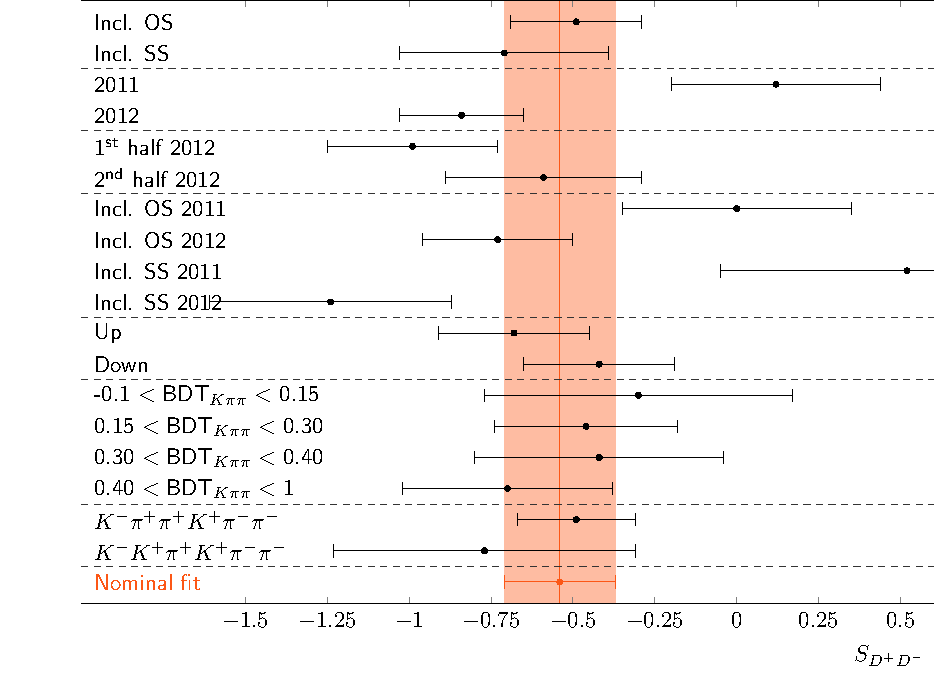
\includegraphics[width=0.9\textwidth]{07-B02DD/tikz/pdf/SComparison.pdf}
\caption{
Comparison of fit results of \SDD for fits on various subsamples.}
\label{fig:b02dd:systematics:xchecks:subsamples:s}
\end{figure}
\begin{figure}[thb]
\centering
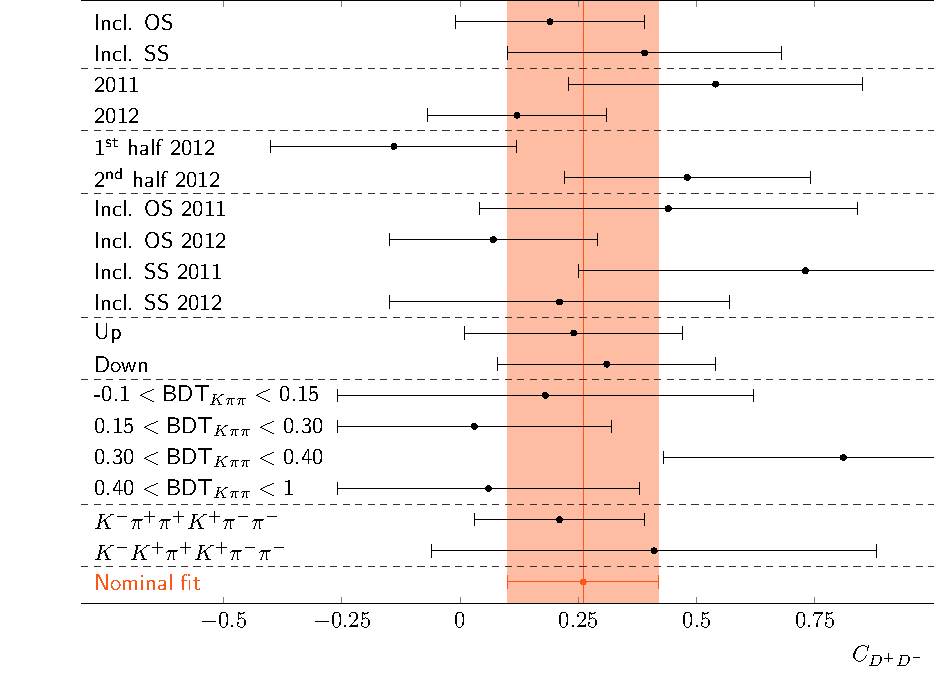
\includegraphics[width=0.9\textwidth]{07-B02DD/tikz/pdf/CComparison.pdf}
\caption{
Comparison of fit results of \CDD for fits on various subsamples.}
\label{fig:b02dd:systematics:xchecks:subsamples:c}
\end{figure}
The fit results in the various scenarios are illustrated in
\cref{fig:b02dd:systematics:xchecks:subsamples:s,fig:b02dd:systematics:xchecks:subsamples:c}.
While almost all splits show compatible results a rather large difference can
be observed between the 2011 and the 2012 subsample for $\SDD$. This is even
more pronounced when using only SS tagging. When determining the flavour
tagging calibration parameters separately for 2011 and 2012 data small
non-significant differences are observed but these can not explain the
different results of the $\CP$ observables. So the best explanation is that
the difference is due to a statistical fluctuation.

For the nominal fit the decay times and the decay time errors from the DTF are
used. The central values of the $\CP$ observables slightly change when using
the decay time (error) from the LVF, $\SDD = \num{-0.539}$ (LVF) vs.
\num{-0.541} (DTF) and $\CDD = \num{0.266}$ (LVF) vs. \num{0.263} (DTF). But
this difference is clearly below the statistical significance.

\FloatBarrier

%============================================================================%
\subsection{Decay Time Fit Bias}
\label{sec:b02dd:systematics:fitbias}

The likelihood fit itself might be biased. The nominal fit results for the
$\CP$ observables are used to generate \num{10000} pseudoexperiments. The pull
distributions in \cref{fig:b02dd:systematics:fitbias:pulls} show a very small
deviation of the mean value from zero.
%
\begin{figure}[htb]
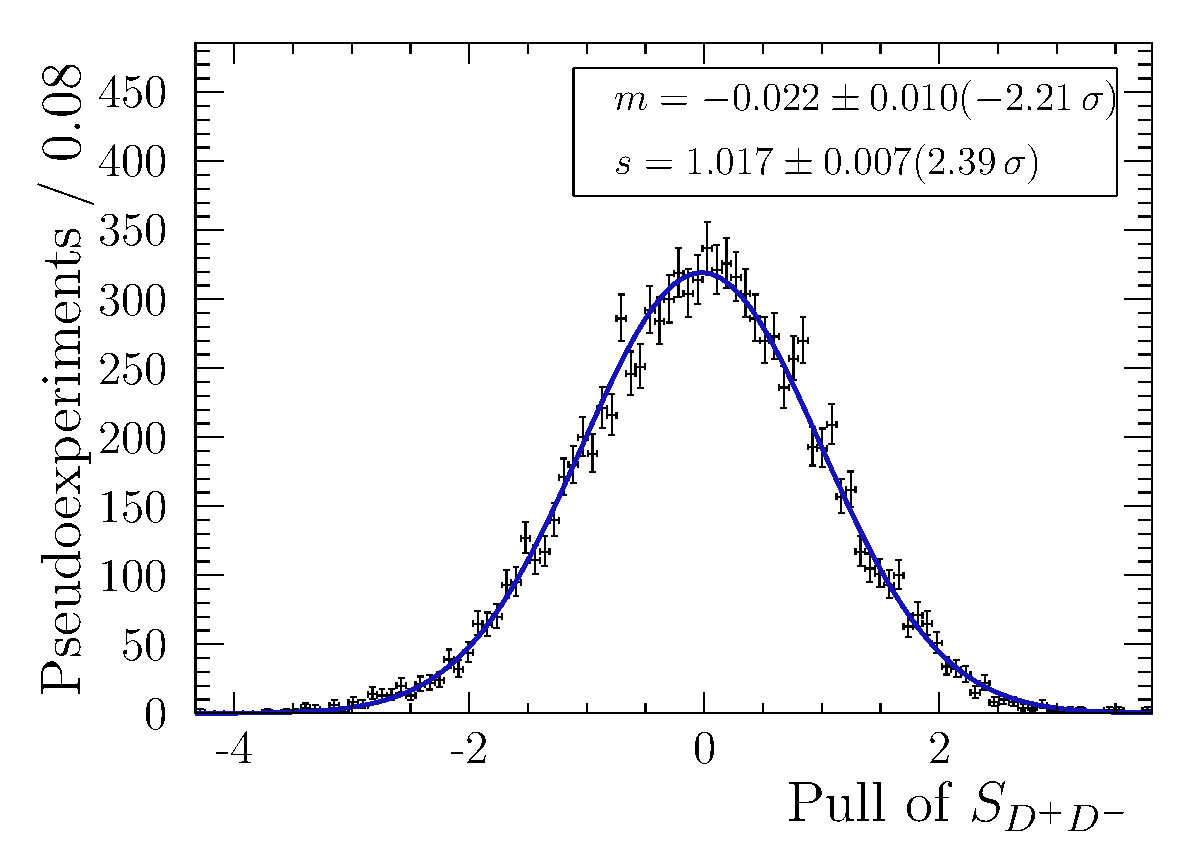
\includegraphics[width=0.49\textwidth]{07-B02DD/tikz/pdf/parSigTimeSin2b_pull_fitbias.pdf}
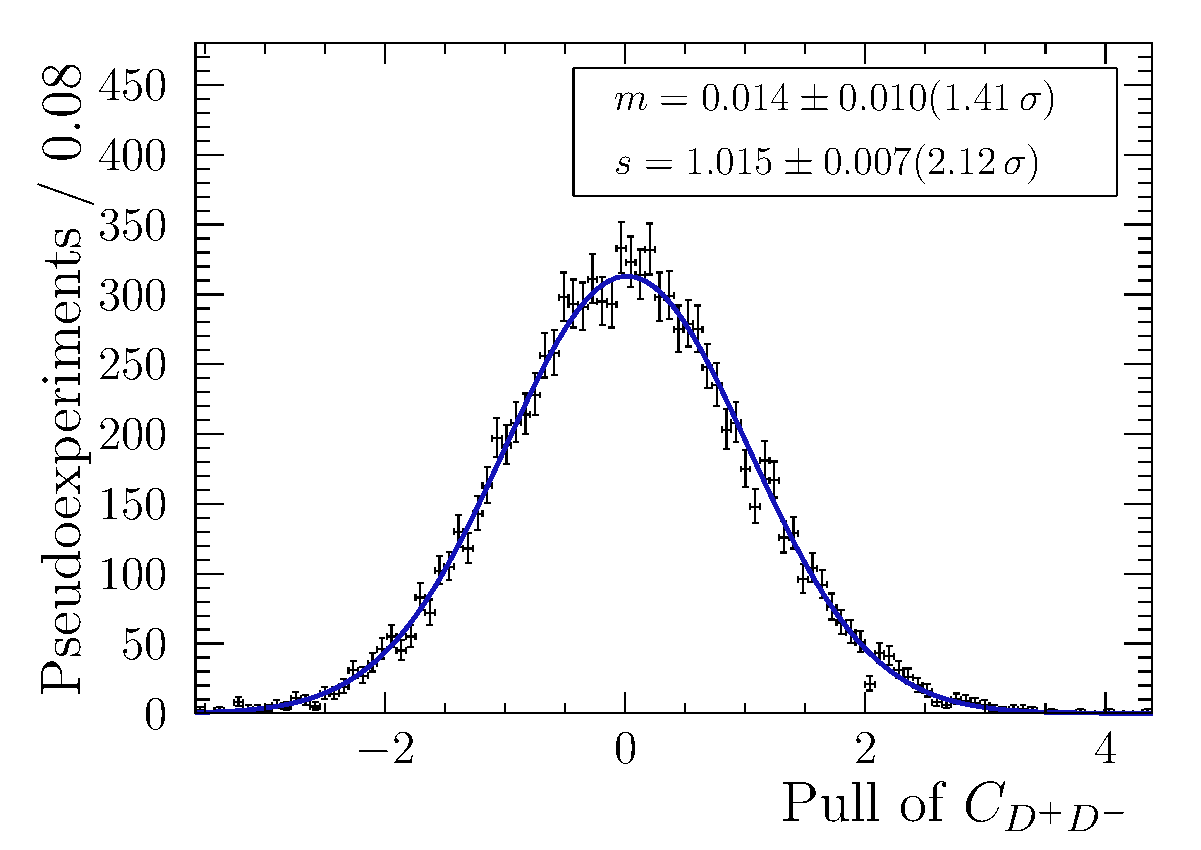
\includegraphics[width=0.49\textwidth]{07-B02DD/tikz/pdf/parSigTimeC_pull_fitbias.pdf}
\caption{Pull distributions of $\SDD$ and $\CDD$ for a study on the systematic
uncertainty due to the likelihood fitter.}
\label{fig:b02dd:systematics:fitbias:pulls}
\end{figure}
%
Multiplying it with the statistical uncertainty the systematic uncertainty is
calculated to be
\begin{align}
s_{\SDD}^{\textrm{fit}} = \num{0.004}\ , \qquad s_{\CDD}^{\textrm{fit}} = \num{0.0025}\ .
\end{align}
For all following studies of systematic uncertainties the residuals are
corrected for the decay time fit bias. Otherwise, even effects that are
actually not biasing would be misinterpreted due to the fit bias.

%============================================================================%
\subsection{Fit Model}
\label{sec:b02dd:systematics:fitmodel}
%!TEX root = ../main.tex

%----------------------------------------------------------------------------%
\subsubsection{Mass Model}
\label{sec:b02dd:systematics:massmodel}

Two different aspects of the mass model are studied regarding systematic
uncertainties: the impact of neglecting contributions and of mismodelling
components.

\paragraph{Neglected contributions}

If a neutral \piz or a photon is missed in the reconstruction the decay
\BToDstD, with \DstpToDpizero or \DstpToDgamma, can mimic the \BToDD decay. In
the rest frame of the \Dstarp resonance, the missing momentum of the \piz is
fixed, but it needs to be boosted when transferred into the rest frame of the
\PB meson. So, the reconstructed mass depends on the helicity angle of the
missing \piz. This leads to a double-horned structure approximately
\SI{140}{\MeVcc} below the nominal \PB mass (see Ref.~\cite{LHCb-ANA-2014-015}
for more details on the shape of this background). As the lower boundary on
the invariant $m_{\Dp\Dm}$ mass is set to \SI{5150}{\MeVcc} the \BdToDstD
contribution lies outside the mass range used for the fit. However, the
\BsToDstD contribution enters the fit region. But since the expected number of
\BsToDstD candidates is low, it is not included in the nominal mass model.
Another contribution that is neglected in the nominal mass fit model is
(partially) charmless background where at least one of the hadron triplets is
not originating from a \PD decay. The systematic uncertainty on the
determination of the \CP observables arising from neglecting these two
contributions is estimated using \num{1000} pseudoexperiments. Components for
\BsToDstD and for (partially) charmless background are included in the
generation but excluded from the fit procedure.

The shape of \BsToDstD is parametrised with two single Gaussian functions
centred around \SI{5150}{\MeVcc} and \SI{5200}{\MeVcc}. The (partially)
charmless background is modelled with a single Gaussian function. When
optimising the decay time significance cut it has been observed that the width
of the (partially) charmless background is approximately \SI{10}{\percent}
wider than the signal component. Therefore, a width of \SI{10}{\MeVcc} is
chosen. The mean is set to the same position as the \Bd signal. The \BsToDstD
component is generated without any tagging asymmetry, while for the (partially)
charmless background the worst case scenario of maximal \CP violation with the
opposite \CP eigenvalue ($S_f = \num{+1.0}$) is tested.

In studies of \BdToDstD decays~\cite{BToDstDthesis} a significant contribution
of \BsToDstD candidates is observed. The ratio between the two yields is
determined to be 1:20. Under the assumption that the efficiencies for \BToDD
and \BToDstD are the same the expected number of \BsToDstD candidates can be
calculated via
\begin{align}
	\text{N}_{\BsToDstD} = \frac{1}{20} \text{N}_{\BdToDD} \frac{\mathcal{B}(\BdToDstD) \mathcal{B}(\Dstarp \!\to \Dp (\piz || \gamma))}{\mathcal{B}(\BdToDD)} \,.
\end{align}
Using the world averages for the branching ratios~\cite{PDG2016} the number of
candidates to be generated in the pseudoexperiments is estimated to be
N(\BsToDstD) = \num{66\pm9}.

To determine how many (partially) charmless background candidates need to be
generated the $D$ mass window is widened to $\SI{\pm40}{\MeVcc}$ and the
nominal $D$ mass window of $\SI{\pm25}{\MeVcc}$ is vetoed for one or for both
$D$ candidates. Fits to the invariant $B$ mass without the $D$ mass constraint
are performed in the various scenarios. % yielding
% $\num{0.0\pm2.6}\,\mbox{\Bd\!\to\KpipiKpipi}$ candidates,
% $\num{0.0\pm9.2}\,\mbox{\Bd\!\to\KKpiKpipi}$ candidates,
% $\num{0.0\pm4.9}\,\mbox{\Bd\!\to\D(\Kpipi)\Kpipi}$ candidates,
% $\num{0.0\pm3.3}\,\mbox{\Bd\!\to\D(\KKpi)\Kpipi}$ candidates, and
% $\num{17.2\pm11.2}\,\mbox{\Bd\!\to\D(\Kpipi)\KKpi}$ candidates.
%
The fitted yields, which are constrained to positive values, are scaled to
account for the applied $D$ mass window. The total amount of residual
contamination ($\Bz\!\to\PD hhh$ or $\Bz\!\to hhhhhh$ decays) surviving the
\BdToDD selection is found to be $\num{28.7\pm19.5}$ candidates for the
$\KKpiKpipi$ final state and $\num{0.0\pm27.8}$ candidates for the
$\KpipiKpipi$ final state. For the pseudoexperiments the number of (partially)
charmless background is drawn from Gaussian distributions using these values
for mean and width. When the outcome is negative the procedure is repeated,
until a positive yield is drawn.

The systematic uncertainties on \SDD and \CDD are calculated as the product of
the bias on the mean parameter of the pull distributions and the statistical
uncertainty:
\begin{align*}
s_{\SDD}^{\text{mass,1}} = \num{0.05}\ , \qquad s_{\CDD}^{\text{mass,1}} = \num{0.013}\,.
\end{align*}

\paragraph{Mismodelling of mass components}

The BDT is trained with MC samples that are known to not perfectly model the
PID information. As a result the BDT classifier distributions of
background-subtracted data and MC show a quite big discrepancy. Some shape
parameters are estimated on MC samples and might be distorted by the data/MC
differences. Therefore, different alternative mass parametrisations are tested
against the nominal model: the component of the \BdToDD signal (and of the
\BsToDD background) is parametrised with a single Gaussian function; the
combinatorial background is described with a second order Chebyshev polynomial
of first kind; the tail parameters of \BToDsD are once extracted from the MC
sample without applying the BDT and once applying a tight cut on the BDT
classifier. The mass fit is performed with these new models, sWeights are
calculated for each approach, and the decay time fit is performed. The results
of the \CP observables are then compared with the nominal central values. The
largest deviations for \SDD and \CDD are
\begin{align*}
s_{\SDD}^{\text{mass,2}} = \num{0.004}\ , \qquad s_{\CDD}^{\text{mass,2}} = \num{0.006}\,.
\end{align*}

%----------------------------------------------------------------------------%
\subsubsection{Correlation between decay time and mistags}
\label{sec:b02dd:systematics:correlation_mistag_time}

The correlation between the decay time distribution and the per-event mistags
is studied by calculating the linear Pearson correlation coefficient
$\rho(\eta,t)$. The significance of the correlation value, \ie
\SI{95}{\percent} confidence level interval, is determined using the
bootstrapping method (\cref{sec:dataanalysis:bootstrapping}) with \num{10000}
repetitions. The correlation coefficients are found to be small. The profile
histogram of the OS tagging combination, which shows the average \etaos value
as a function of the decay time, is flat within statistics. For the SS tagging
combination the profile histogram slowly increases with decay time. This can
be confirmed by analysing the larger signal MC sample (see
\cref{fig:b02dd:systematics:correlation_mistag_time:etass_time_profile_MC}).
\begin{figure}[htb]
\centering
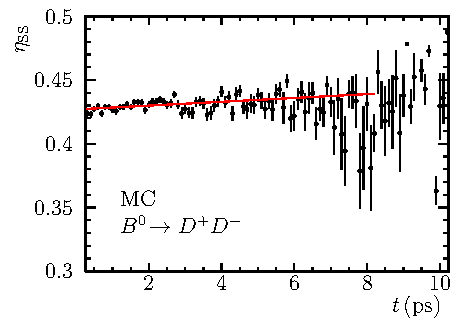
\includegraphics[width=0.6\textwidth]{07-B02DD/tikz/pdf/Profile_DecayTime_SS.pdf}
\caption{Profile histogram for the decay time dependence on $\etass$ for
signal MC. The black data points represent the mean value of $\etass$ and its
uncertainty for each bin in $t$. The red curve is the fitted linear function.}
\label{fig:b02dd:systematics:correlation_mistag_time:etass_time_profile_MC}
\end{figure}
Performing a $\chisq$ fit in the decay time range \SIrange{0.25}{8.25}{\ps}
with the linear function
\begin{align}
  \etass = a_{\etass,t} t + b_{\etass,t}
  \label{eq:tagging:correlation_mistag_time}
\end{align}
yields a slope of $a_{\etass,t} = \SI{1.50\pm0.27}{\invns}$. Although this is
a significant deviation from zero, the correlation is not taken into account in
the nominal fit model. Instead, a study on the systematic uncertainty from
neglecting this effect is performed. In \num{1000} pseudoexperiments the SS
mistag is generated using a Gaussian distribution whose mean is drawn from the
linear function defined in \cref{eq:tagging:correlation_mistag_time} thereby
introducing the correlation with the decay time. In the subsequent fit the
correlation is again ignored. This leads to systematic uncertainties of
\begin{align*}
s_{\SDD}^{\text{corr}} = \num{0.0007}\ , \qquad s_{\CDD}^{\text{corr}} = \num{0.007}\,.
\end{align*}

%----------------------------------------------------------------------------%
\subsubsection{Decay Time Resolution Model}
\label{sec:systematics:decaytimeresolution}

As calculated in \cref{sec:b02dd:decaytimefit:resolution} even an
underestimation of the decay time resolution by \SI{15}{\percent} has only a
minor effect on the resolution related dilution. Nevertheless, \num{1000}
pseudoexperiments are performed, in which the scale factors and the offset
parameters ($b_i$ and $c_i$ from \cref{tab:b02dd:decaytimefit:resolution}) are
enlarged by \SI{15}{\percent} in the generation and fixed to their nominal
values in the fit. Additionally, the mean parameter of the Gaussians is set to
the value obtained in the MC study for the generation and, like in the nominal
setup, fixed to zero in the fit. The systematic uncertainties are calculated
as the product of the biases on the mean parameter and the statistical
uncertainty to be
\begin{align*}
s_{\SDD}^{\text{res}} = \num{0.0020}\ , \qquad s_{\CDD}^{\text{res}} = \num{0.0023}\,.
\end{align*}

%----------------------------------------------------------------------------%
\subsubsection{Decay Time Acceptance Model}
\label{sec:systematics:decaytimeacceptance}

On signal MC the decay time acceptance is determined separately for the two
final states (see \cref{fig:b02dd:decaytimefit:acceptance_MC}). Small
differences are observed. As the low statistics in the \KKpiKpipi final state
on data does not allow for an individual spline model, a study is performed to
estimate a possible systematic uncertainty from neglecting this difference. In
\num{1000} pseudoexperiments the decay time distribution is generated using
the histograms of the true decay time acceptance from signal MC, split by
final state, and fitted with the spline acceptance as done in the nominal fit.
The use of the histograms with \num{100} bins should also cover uncertainties
from the choice of the number and position of the knots. The pull between the
fit results and the generation values is calculated. The systematic
uncertainty due to the decay time acceptance model is calculated as the
product of the shift in the pull distribution and the statistical uncertainty
of the nominal fit:
\begin{align*}
s_{\SDD}^{\textrm{acc}} = \num{0.007}\ , \qquad s_{\CDD}^{\textrm{acc}} = \num{0.0027}\,.
\end{align*}


%============================================================================%
\subsection{Further Studies}
\label{sec:b02dd:systematics:others}
%!TEX root = ../main.tex

%----------------------------------------------------------------------------%
\subsubsection[\texorpdfstring{$z$}{z}-scale]{\texorpdfstring{$\boldsymbol{z}$}{z}-scale}
\label{sec:b02dd:systematics:z_scale}

The decay times are determined by measuring the distance between PV and decay
vertex. So, any uncertainty on the positioning of detector elements
(especially the VELO modules) leads to biased decay times. Due to the high
boosting the main contribution to the flight distance is in $z$ direction. The
scale uncertainty in $z$ direction has been estimated to be
$\sigma_{z\text{-scale}} = \SI{0.022}{\percent}$~\cite{LHCb-ANA-2011-055}. The
influence on the measurement of the \CP observables is studied by performing
\num{1000} pseudoexperiments. For each pseudoexperiment a value for the uncertainty
on the $z$-scale is drawn from a Gaussian distribution around zero of width
$\sigma_{z\text{-scale}}$. The sum of \SI{50}{\fs} and the product of this
value with the decay time is used as width of the Gaussian function modelling
the decay time resolution in the generation. In the fit the width is set to
\SI{50}{\fs}. The product of the bias from the pull distributions of the
pseudoexperiments and the nominal statistical uncertainty is taken as
systematic uncertainty:
\begin{align*}
s_{\SDD}^{z\text{-scale}} = \num{0.0031}\ , \qquad s_{\CDD}^{z\text{-scale}} = \num{0.0028}\,.
\end{align*}

%----------------------------------------------------------------------------%
\subsubsection{Production Asymmetry}
\label{sec:b02dd:systematics:production_asymmetry}

The systematic uncertainty on the production asymmetry \prodasym{11} is
studied using \num{1000} pseudoexperiments. The nominal value is used in the
generation and the procedure described in Ref.~\cite{Karbach:1490463} is
applied in the fit: Before fitting the data sample the mean of the Gaussian
constraint for \prodasym{11} is shifted by one systematic uncertainty. The
resulting Gaussian distribution is used to draw a new value for the mean.
Then, the new Gaussian distribution is used to constrain \prodasym{11} in the
fit. Both shifts, upwards and downwards, are tested and the larger deviation
is taken as systematic uncertainty:
%
\begin{align*}
s_{\SDD}^{\prodasym{}} = \num{0.0015}\ , \qquad s_{\CDD}^{\prodasym{}} = \num{0.004}\,.
\end{align*}
%
For the production asymmetry difference $\Delta\prodasym{}$ the systematic
uncertainty is already included in the Gaussian constraint of the nominal fit.

%----------------------------------------------------------------------------%
\subsubsection{Decay Width Difference \texorpdfstring{\DGd}{Delta Gamma\_d}}
\label{sec:b02dd:systematics:deltagammad}

The decay width difference \DGd is expected to be very small and therefore
fixed to zero in the nominal fit. But experimentally it has a relatively large
uncertainty. This is taken into account by performing \num{1000}
pseudoexperiments where the current statistical precision $\sigma(\DGd) =
\SI{\pm0.007}{\invps}$~\cite{HFAG} is used in the generation of the data
samples while it is, like in the nominal model, neglected in the fit. The mean
parameters of the pull distributions are converted into systematic
uncertainties of
\begin{align*}
s_{\SDD}^{\DGd} = \num{0.014}\ , \qquad s_{\CDD}^{\DGd} = \num{0.0021}\,.
\end{align*}

%----------------------------------------------------------------------------%
\subsubsection{\texorpdfstring{$\Bz$}{B0} Mass Difference \texorpdfstring{\dmd}{Delta m\_d}}
\label{sec:b02dd:systematics:deltamd}

The systematic uncertainty on the world average of \dmd
($\SI{\pm0.002}{\hbar\invps}$~\cite{HFAG}) is not covered by the Gaussian constraint that
is used in the nominal fit. Instead, it is analysed using \num{1000}
pseudoexperiments. In the generation the nominal model is used. Before
performing the fit the mean of the Gaussian distribution (its width is the
statistical precision of the world average) is shifted by one systematic
uncertainty (once up and once down) and a new value is drawn from the
distribution. This new constraint is then used in the minimisation. Looking at
the resulting pull distributions systematic uncertainties of
\begin{align*}
s_{\SDD}^{\dmd} = \num{0.0025}\ , \qquad s_{\CDD}^{\dmd} = \num{0.006}\,,
\end{align*}
are assigned.


% \FloatBarrier
%============================================================================%
\subsection{Total Systematic Uncertainty}
\label{sec:b02dd:systematics:total}

The systematic uncertainties are summarised in
\cref{tab:b02dd:systematics:total}. The full systematic uncertainty is
calculated by summing the individual uncertainties in quadrature.
%
\begin{table}[!htb]
\caption{Systematic uncertainties on the $\CP$ observables $\SDD$ and $\CDD$.}
\label{tab:b02dd:systematics:total}
  \centering
    \begin{tabular}{lSS}
      \toprule
      Origin & {\param{\sigma}{}{$\SDD$}} & {\param{\sigma}{}{$\CDD$}}    \\
      \midrule
      Neglecting components in mass model     &  0.05    & 0.013  \\
      $\DGd$                                  &  0.014   & 0.0021 \\
      Decay time acceptance                   &  0.007   & 0.0027 \\
      Correlation between mass and decay time &  0.0007  & 0.007  \\
      Parametrisation of PDFs in mass model   &  0.004   & 0.006  \\
      $\dmd$                                  &  0.0025  & 0.006  \\
      Fit bias                                &  0.004   & 0.0025 \\
      Production asymmetry                    &  0.0015  & 0.004  \\
      $z$-scale                               &  0.0031  & 0.0028 \\
      Decay time resolution                   &  0.0020  & 0.0023 \\
      \midrule
      Sum                                     &  0.05    & 0.018  \\
      \bottomrule
    \end{tabular}
\end{table}